% !TeX spellcheck = hr-HR
\documentclass[diplomskirad, upload]{fer}

\usepackage{booktabs}
\usepackage{graphicx}
\usepackage{listings}
\usepackage{courier}
\usepackage{xcolor}
\usepackage{subcaption}
\usepackage{float}
 	
\definecolor{lightGray}{HTML}{F0F0F0}

\lstset{
	basicstyle=\ttfamily\footnotesize,
	breaklines=true,
	showstringspaces=false,
	tabsize=2,
	backgroundcolor = \color{lightGray},
	framexleftmargin=10pt,
	framexrightmargin=10pt,
	keywords={abstract, continue, for, new, switch, assert, default, goto, 
		package, synchronized, boolean, do, if, private, this, 
		break, double, implements, protected, throw, byte, else, 
		import, public, throws, case, enum, instanceof, return, 
		transient, catch, extends, int, short, try, char, final, 
		interface, static, void, class, finally, long, strictfp, 
		volatile, const, float, native, super, while},
	sensitive=true,
	comment=[l]{//},
	morecomment=[s]{/*}{*/},
	morestring=[b]",
	morestring=[b]',
	keywordstyle=\color{blue},
	stringstyle=\color{red},
	commentstyle=\color{green},
}

\graphicspath{ {./figures/} }


%---------------------------- Title page ----------------------------------

\begin{document}

\title{Application to assist with learning to play the piano}

\naslov{Aplikacija za pomoć učenju sviranja klavira}

\brojrada{675}

\author{Ana Bagić}

\mentor{Prof.\@ Marko Čupić}

\date{September, 2024}

\datum{rujan, 2024.}

\maketitle


%---------------------------- Assignment page -----------------------------

\zadatak{zadatak.pdf}


%---------------------------- Thank you page ------------------------------

\begin{zahvale}
\end{zahvale}


\mainmatter


%---------------------------- Contents section ----------------------------

\tableofcontents


%---------------------------- Introduction section ------------------------

\chapter{Uvod}
Učenje sviranja klavira složen je proces koji od učenika zahtijeva koordinaciju niza kognitivnih i motoričkih vještina, uključujući sinkronizaciju pokreta obje ruke, precizno usklađivanje ritma, kontrolu dinamike, te istovremeno čitanje i razumijevanje notnog zapisa. Ovi zadaci mogu biti prilično zahtjevni, posebno za početnike, koji često moraju savladati više aspekata u isto vrijeme.

U današnjem digitalnom dobu, računalne aplikacije nude značajnu pomoć u procesu učenja sviranja raznih instrumenata, a zbog njegove popularnosti, najčešće klavira. One pružaju vizualne i zvučne povratne informacije koje pomažu učenicima u prepoznavanju i ispravljanju grešaka, praćenju napretka i usavršavanju tehnike sviranja. One također omogućuju interaktivni i personalizirani pristup učenju i mogu značajno unaprijediti učinkovitost, zadovoljstvo i zabavu u procesu učenja. Iako ove aplikacije ne mogu u potpunosti zamijeniti iskusne učitelje i tradicionalne škole, one su pristupačnije široj publici i omogućuju neformalno i fleksibilno učenje. Neke od aplikacija usmjerene su na poučavanje teorije glazbe, neke na praktične elemente, ali većina njih na neki način kombinira oba pristupa.

U ovom diplomskom radu istražila sam kako se računalne tehnologije mogu koristiti za nadopunu tradicionalnih metoda, s ciljem olakšavanja procesa učenja sviranja klavira. Razvila sam aplikaciju koja koristi praktičan pristup, specifično uči korisnika svirati odabranu skladbu. Ona na dva načina prikazuje što treba odsvirati: pomičnim notnim zapisom i bojom istaknutim tipkama klavira, te analizom odsviranog prati uspješnost korisnika. U radu sam predstavila svoje programsko rješenje, prikazala postignute rezultate, analizirala njegove prednosti i nedostatke, te navela ideje za poboljšanje i nadogradnju. Uz rad priložen je izvorni i izvršni kod razvijenog programa.


%---------------------------- Problem description section -----------------

\chapter{Opis problema}
Cilj ovog diplomskog rada je razviti aplikaciju koja korisnicima omogućuje učinkovito učenje sviranja odabranih skladbi kombinirajući tradicionalne metode s modernim tehnologijama. Korisnik u aplikaciji odabire skladbu u MusicXML formatu (detaljno objašnjen u odjeljku \ref{sec:musicxml}) koju želi savladati, dok mu aplikacija istovremeno nudi dvije različite vizualne reprezentacije onoga što treba odsvirati: pomični notni zapis i vizualno istaknute tipke na klaviru. Aplikacija kontinuirano prati korisnikovu izvedbu putem klavijature povezane s računalom MIDI protokolom (detaljno objašnjeno u odjeljku \ref{sec:midi}), analizira njegov napredak i daje povratne informacije o točnosti sviranja odabrane skladbe. Ovaj rad fokusira se na razvoj aplikacije koja pojednostavljuje proces učenja sviranja, čineći ga interaktivnim i pristupačnim.

U nastavku ovog poglavlja bit će predstavljene postojeće slične aplikacije, zajedno s njihovim značajkama i mogućnostima, te usporedba s programskim rješenjem razvijenim u ovom radu, kako bi se definirale ključne razlike između njih.

\section{Postojeće aplikacije}
Postoji veliki broj aplikacija koje se bave sličnom tematikom, međutim u nastavku navesti ću neke od najpoznatijih i najkorištenijih.

\subsection{Synthesia}
Synthesia \cite{synthesia} je aplikacija koja korisnicima omogućuje sviranje skladbi uz pomoć vizualnih uputa na ekranu. Osim za učenje, mnogi glazbenici koriste ju za digitalizaciju i prikaz svojih skladbi ili aranžmana tuđih, a na Youtube-u se često mogu vidjeti videozapisi izrađeni pomoću te aplikacije. Note se prikazuju u obliku padajućih blokova iznad klavijature, pomažući korisnicima da prate koje tipke treba pritisnuti, što je prikazano na slici \ref{fig:synthesia}. Osim bogate biblioteke pjesama koju sadrži, Synthesia podržava i učitavanje MIDI datoteka, omogućujući korisnicima sviranje raznih skladbi. Aplikacija također prati korisnikov napredak, omogućuje prilagodbu tempa i vježbanje specifičnih dijelova skladbe, što je korisno za početnike i samouke glazbenike.

\begin{figure}[h]
	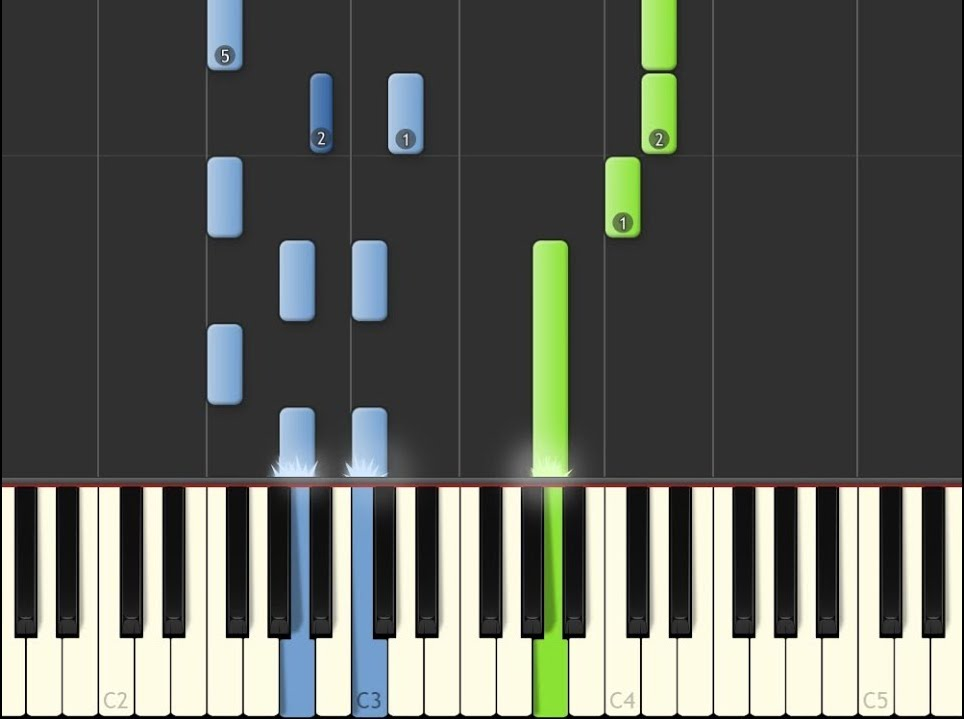
\includegraphics[width=\textwidth]{synthesia.jpg}
	\centering
	\caption{Synthesia \cite{synthesia}}
	\label{fig:synthesia}
\end{figure}

Slično mojoj aplikaciji, Synthesia koristi bojom istaknute tipke na klaviru, ali se više oslanja na prikaz padajućih nota umjesto na tradicionalni notni zapis. Obje aplikacije nude praćenje korisnikove izvedbe na povezanoj klavijaturi i pružaju povratne informacije. Međutim, dok Synthesia nudi učitavanje isključivo MIDI datoteka, moja aplikacija koristi MusicXML format koji omogućuje precizniji prikaz notnog zapisa.

\subsection{Simply Piano}
Simply Piano \cite{simplypiano} je popularna mobilna aplikacija za učenje sviranja klavira koja nudi interaktivne lekcije i vježbe prilagođene različitim razinama vještine, a primjer korištenja može se vidjeti na slici \ref{fig:simplypiano}. Korisnici mogu učiti skladbe iz opsežnog kataloga pjesama, a aplikacija koristi tehnologiju prepoznavanja zvuka za analizu izvedbe i pružanje povratne informacije u stvarnom vremenu. S obzirom da ta metoda nije skroz ispravna kod određivanja odsviranih nota, od nedavno Simply Piano podržava i praćenje korisnika putem MIDI protokola kao i moja aplikacija, međutim pošto je namijenjena isključivo mobilnim uređajima, spajanje klavijature na uređaj može biti složenije. Moja aplikacija također omogućuje učitavanje skladbi u MusicXML formatu, dok Simply Piano podržava samo pjesme iz svog kataloga.

\begin{figure}[h]
	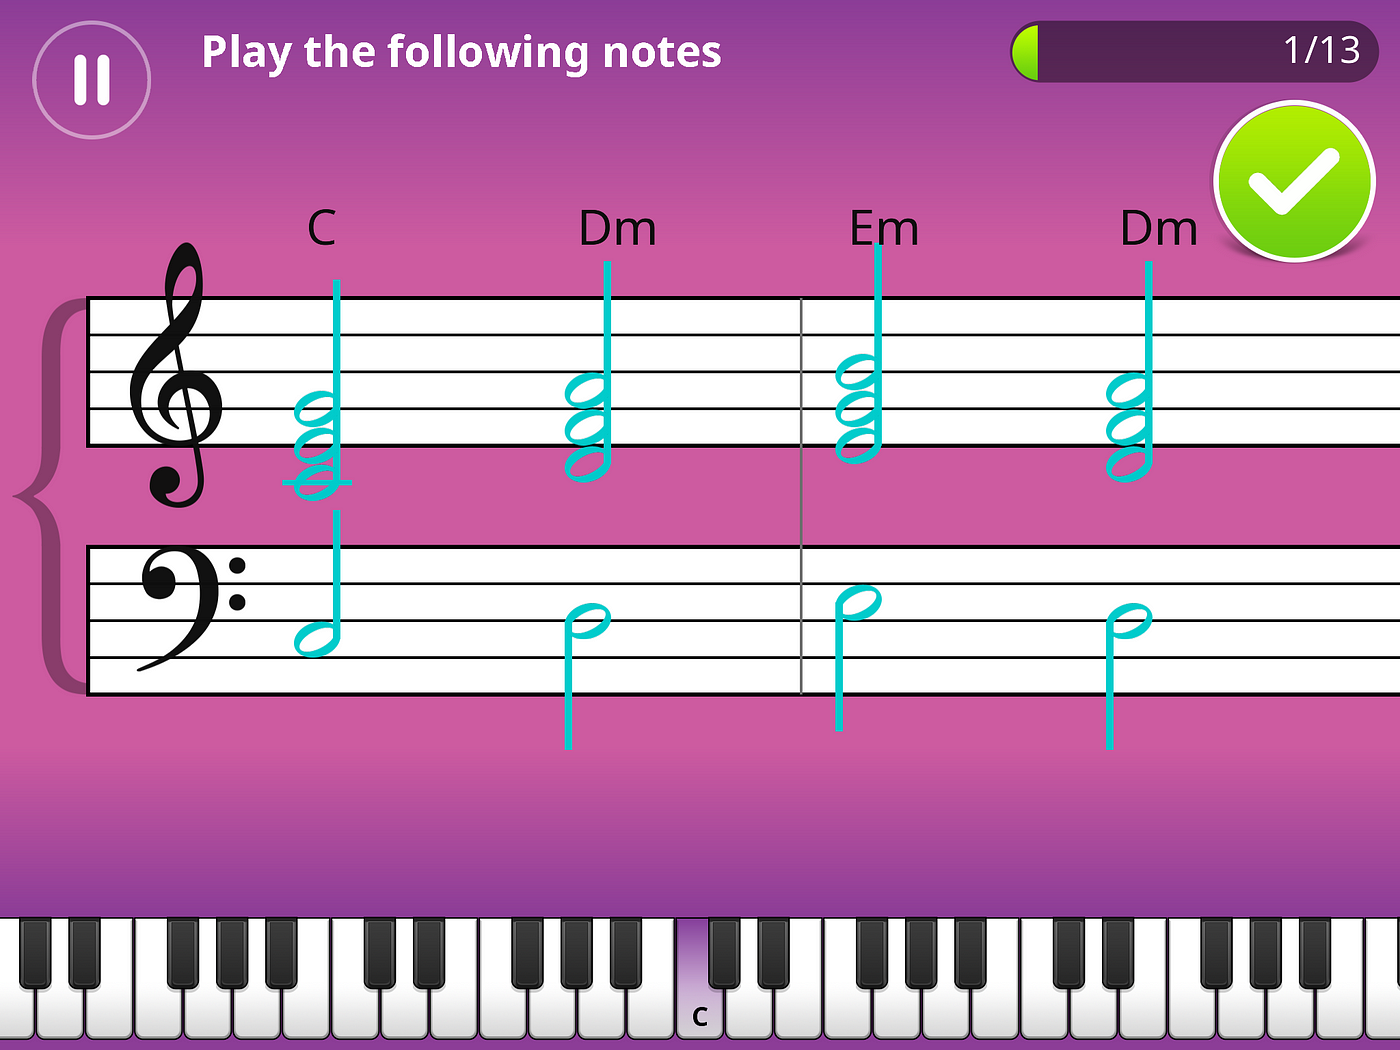
\includegraphics[width=\textwidth]{simply-piano.png}
	\centering
	\caption{Simply Piano \cite{simplypianoimage}}
	\label{fig:simplypiano}
\end{figure}

\subsection{Flowkey}
Flowkey \cite{flowkey} je aplikacija za učenje sviranja klavira koja kombinira interaktivne lekcije, i širok katalog skladbi. Primjer korištenja prikazan je na slici \ref{fig:flowkey}. Aplikacija omogućuje korisnicima učenje sviranja pjesama uz pomoć video vodiča (engl. \textit{tutorial}) i dinamičkih prikaza notnih zapisa. Koristi tehnologiju prepoznavanja zvuka, kao i MIDI vezu s računalom kako bi analizirala korisnikovu izvedbu u stvarnom vremenu i pružala povratne informacije.

Flowkey nudi različite razine težine, od početnika do naprednih korisnika, te omogućuje odabir specifičnih dijelova skladbe za vježbanje, što moja aplikacija trenutno ne podržava. Aplikacija je dostupna na više platformi, uključujući mobilne uređaje i računala, što olakšava pristup različitim korisnicima. Za razliku od moje aplikacije, Flowkey ne podržava učitavanje vlastitih skladbi, što može biti ograničenje za korisnike koji žele raditi s notnim zapisima izvan Flowkey biblioteke.

\begin{figure}[h]
	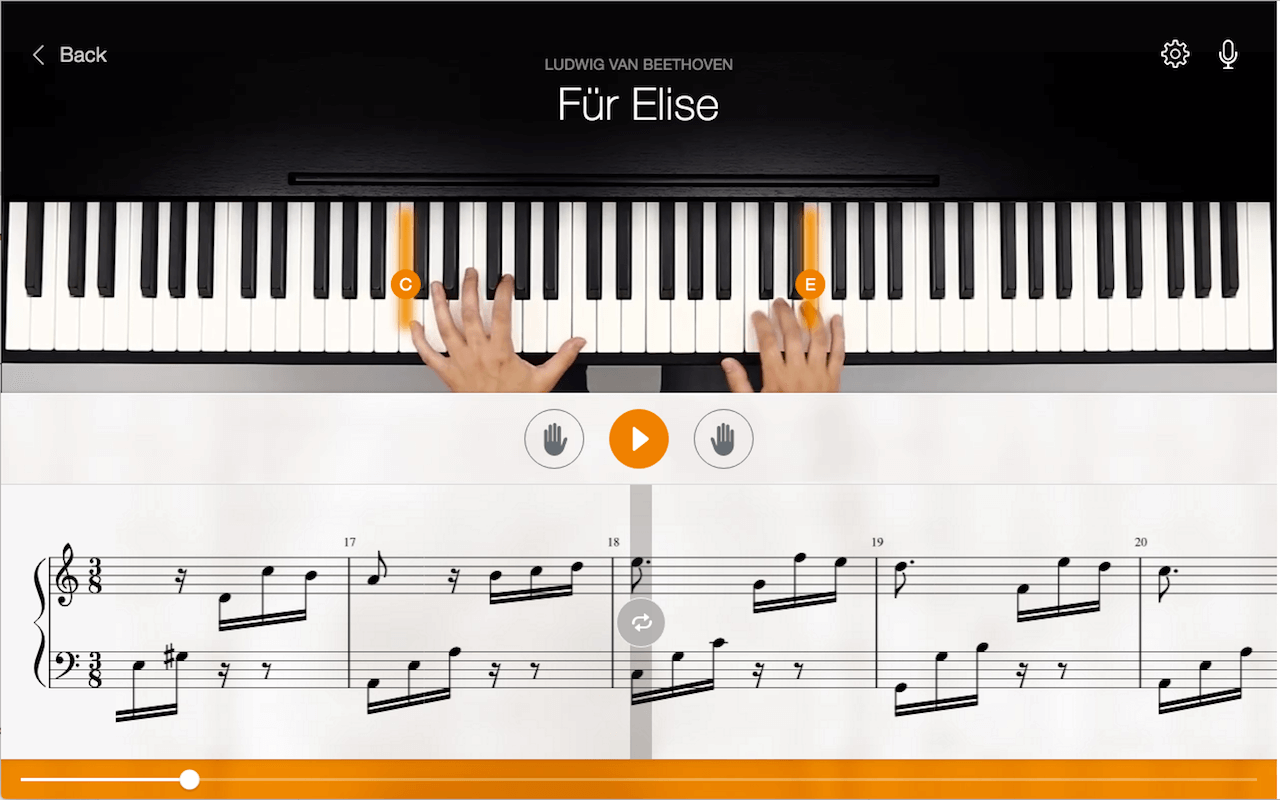
\includegraphics[width=\textwidth]{flowkey.png}
	\centering
	\caption{Flowkey \cite{flowkeyimage}}
	\label{fig:flowkey}
\end{figure}


%---------------------------- Used technologies section -------------------

\chapter{Korištene tehnologije}
Aplikaciju za učenje sviranja klavira razvila sam koristeći Javu 21, trenutno (kolovoz 2024.) najnoviju verziju programskog jezika s dugoročnom podrškom (engl. \textit{LTS}). Upravljanje projektom ostvarila sam putem Apache Maven alata, dok sam za izradu korisničkog sučelja koristila JavaFX biblioteku. Kao ulazni format datoteka upotrijebila sam MusicXML, koji sam deserijalizirala pomoću ProxyMusic biblioteke. Za prepoznavanje unosa s klavijature i reprodukciju glazbe koristila sam MIDI protokol, a prikaz notnog zapisa olakšala sam si korištenjem Bravura fonta, koji slijedi SMuFL specifikaciju.

U nastavku ovog poglavlja navesti ću osnovne informacije o navedenim tehnologijama i objasniti njihovu primjenu u ovom projektu.

\section{Apache Maven}
Maven \cite{maven} je alat za upravljanje programskim projektima i automatizaciju izgradnje. Razvijen je od strane Apache Software Foundationa, a prvi put je pušten u rad u srpnju 2004. godine. Prvenstveno je dizajniran za Java projekte, ali može se upotrijebiti i za rad u drugim programskim jezicima kao što su C\#, Scala, Ruby i drugi. Jedna od ključnih značajki Mavena je njegova sposobnost za automatsko upravljanje procesom izgradnje, što uključuje prevođenje koda, izvođenje testova i pakiranje aplikacija. Međutim, možda najvažnija prednost Mavena je njegova funkcionalnost upravljanja ovisnostima (engl. \textit{dependency}) prema vanjskim bibliotekama.

\section{JavaFX}
JavaFX \cite{javafx} je biblioteka razvijena za programski jezik Java, namijenjena izgradnji korisničkih sučelja aplikacija. Razvila ju je kompanija Oracle, a prva verzija objavljena je u prosincu 2008. godine. JavaFX se može koristiti za razvoj desktop, web, mobilnih i ugrađenih (engl. \textit{embedded}) aplikacija.

Jedna od ključnih prednosti JavaFX-a je mogućnost odvajanja logike aplikacije od vizualnog prikaza. Vizualni elementi često se definiraju u FXML datotekama, koje koriste poseban XML format, te u kombinaciji s tim i SceneBuilder – alat koji koristi povuci-i-ispusti (engl. \textit{drag-and-drop}) tehniku za jednostavno kreiranje i uređivanje izgleda aplikacije. Međutim, u svom radu odlučila sam komponente izravno napisati u kodu, bez korištenja FXML-a i SceneBuilder-a. Ovaj pristup mi je omogućio precizniju kontrolu nad izgledom i ponašanjem komponenata, te jednostavniju nadogradnju i jasniji pregled svega što je definirano u kodu kako bi komponenta izgledala na željeni način. JavaFX podržava stiliziranje komponenata putem CSS-a, no tu sam mogućnost koristila jedino kada neki dizajn nije bilo moguće napraviti putem koda.

\section{MusicXML i ProxyMusic}
\label{sec:musicxml}
MusicXML (Music Extensible Markup Language) \cite{musicxml} je format datoteke temeljen na XML specifikaciji, dizajniran za reprezentaciju zapadnjačkog notnog zapisa na način koji je razumljiv i ljudima i računalima. Ovaj format je osmislio Michael Good, a razvila ga je tvrtka Recordare LLC. Prva verzija MusicXML-a objavljena je u siječnju 2004. godine.

MusicXML je danas postao standardni format za digitalni notni zapis, koji koriste brojne aplikacije za kreiranje, reprodukciju i dijeljenje notnog zapisa. Mnoge od tih aplikacija omogućuju učitavanje datoteka u MusicXML formatu, uređivanje notnog zapisa, reprodukciju te izvoz u različite formate poput PDF-a, XML-a, MIDI-ja, mp3-a i drugih. S vremenom su se mogućnosti i značajke MusicXML-a značajno proširile, tako da sada podržava većinu oznaka i simbola korištenih u klasičnim notnim zapisima.

Struktura MusicXML formata slična je drugim XML formatima. Svaki element u MusicXML-u sastoji se od oznake, opcionalnih atributa u obliku naziv="vrijednost", te opcionalnog sadržaja unutar elementa. Na slici \ref{fig:musicxmlfile} prikazan je primjer MusicXML datoteke koja definira jedan takt u četveročetvrtinskoj mjeri i C-dur ljestvici, unutar kojeg se nalazi jedna cijela nota. Zbog sažetijeg prikaza iz datoteke sam izbacila sve oznake sa metapodatcima. Notni zapis te datoteke može se vidjeti na slici \ref{fig:musicxmlnote}.

S obzirom da tekstualni prikaz MusicXML-a može biti vrlo dugačak, MusicXML v2.0 uvodi komprimirani format sa sufiksom .mxl, koji može smanjiti veličinu datoteka na otprilike jednu dvadesetinu veličine nekomprimirane verzije. Međutim, zbog pojednostavljenja implementacije moja aplikacije ne podržava taj format.

\begin{figure}[h]
	\centering
	\begin{minipage}{0.577\textwidth}
		\centering
		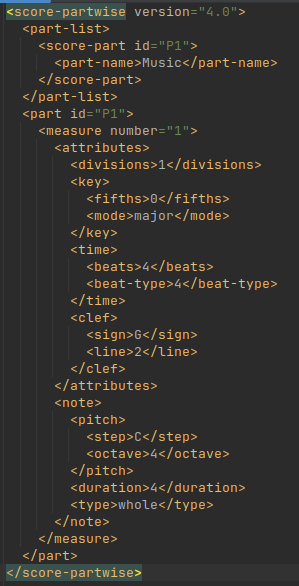
\includegraphics[width=\linewidth]{musicxml-file.png}
		\caption{MusicXML datoteka}
		\label{fig:musicxmlfile}
	\end{minipage}
	\hfill
	\begin{minipage}{0.4\textwidth}
		\centering
		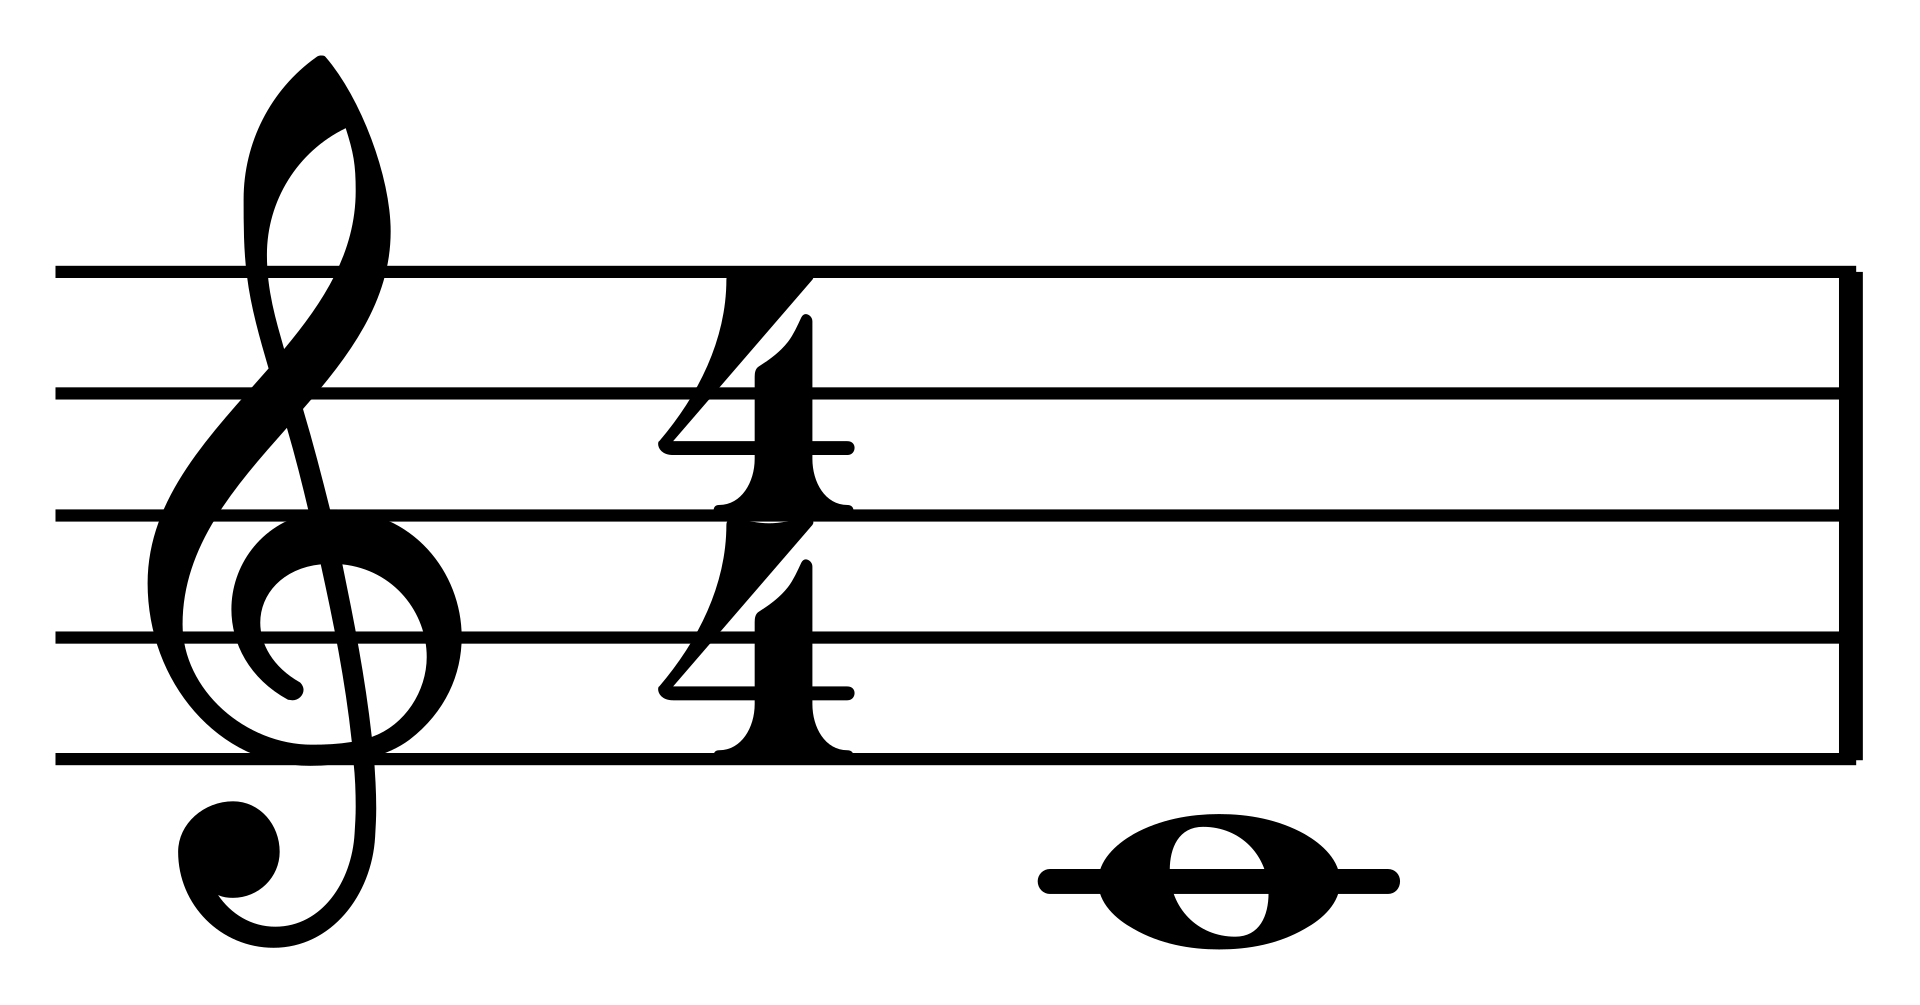
\includegraphics[width=\linewidth]{musicxml-note.png}
		\caption{Notni zapis \cite{musicxml}}
		\label{fig:musicxmlnote}
	\end{minipage}
	\caption{MusicXML primjer}
\end{figure}

MusicXML format sadrži velik broj oznaka i kompleksnih struktura, što ručnu deserijalizaciju čini izuzetno zahtjevnom. Kako bih si to olakšala, koristila sam biblioteku koja automatski obavlja te zadatke. ProxyMusic je biblioteka koja omogućava jednostavnu serijalizaciju, deserijalizaciju i uređivanje MusicXML datoteka, međutim ne nudi nikakve naprednije mogućnosti obrade i analize skladbe. ProxyMusic je osim za Javu, dostupna i za Python, pružajući programerima u oba jezika moćan alat za rad s MusicXML formatom. Upute za preuzimanje biblioteke, kao i dokumentacija i primjeri upotrebe dostupni su na GitHub profilu korisnika \textit{Audiveris} na sljedećoj poveznici \cite{proxymusic}. Biblioteka je također dostupna na Maven repozitoriju i može se pronaći na ovoj poveznici \cite{proxymusicmaven}.

\section{MIDI protokol}
\label{sec:midi}
MIDI (Musical Instrument Digital Interface) \cite{midi} je standardni protokol za povezivanje i komunikaciju između elektroničkih glazbenih instrumenata, računala i drugih uređaja koji se koriste za stvaranje, reprodukciju i obradu glazbe. Razvijen je 1980-ih i prenosi digitalne informacije, poput tona, dinamike i kontrolnih uputa, a ne sam zvuk, što čini MIDI datoteke i poruke malim i učinkovitim. MIDI kabel može prenositi do 16 kanala, a svaki može kontrolirati različite instrumente, što omogućava sinkronizaciju više uređaja u glazbenim sustavima. Njegova standardiziranost osigurava kompatibilnost među različitim uređajima i aplikacijama, čineći ga neophodnim alatom u modernoj glazbenoj industriji. MIDI omogućava preciznu kontrolu i fleksibilnost u stvaranju i reproduciranju glazbe.

Java nativno podržava MIDI putem Java Sound programskog sučelja (engl. \textit{API}), konkretno kroz \textit{javax.sound.midi} paket, koji je jednostavan za korištenje. U svojoj aplikaciji koristila sam MIDI protokol na dva načina: za primanje podataka sa klavijature o tome što korisnik svira i za implementaciju reprodukcije glazbe. Detaljna programska implementacija ovih funkcionalnosti prikazana je u pododjeljcima \ref{sec:mididevices}, \ref{sec:midimessages} i \ref{sec:keyboard}.

Klavijature se mogu spojiti s računalom na dva načina. Većina novijih klavijatura opremljena je USB tip B priključkom (engl. \textit{port}) na stražnjoj strani, a kabel s USB-B priključkom na jednoj strani i USB-A na drugoj lako je dostupan. Međutim, stariji modeli klavijatura, uključujući onu s kojoj sam radila, nemaju USB priključak, nego samo MIDI priključke. Nažalost, kabel s MIDI priključcima, puno je teže pronaći i većina trgovina s glazbenom opremom ga ne nudi. Stoga sam bila prisiljena naručiti ga iz Slovenije.

Na slici \ref{fig:ports} prikazani su spomenuti priključci. S lijeve strane nalaze se MIDI priključci, dok je s desne strane USB-B priključak. Noviji modeli klavijatura sadrže oba priključka, omogućujući korisnicima da odaberu najprikladniji način spajanja. Ako se koriste MIDI priključci, važno je zapamtiti da \textbf{MIDI OUT} priključak na kabelu treba biti povezan s \textbf{MIDI IN} priključkom na klavijaturi, dok \textbf{MIDI IN} na kabelu treba biti povezan s \textbf{MIDI OUT} na klavijaturi. U suprotnom, informacije neće biti prenesene.

\begin{figure}[h]
	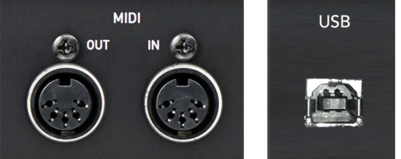
\includegraphics[width=\textwidth]{keyboard-ports.png}
	\centering
	\caption{Priključci na klavijaturi \cite{keyboardports}}
	\label{fig:ports}
\end{figure}

\section{SMuFL specifikacija i Bravura font}
SMuFL (Standard Music Font Layout)\cite{smufl} je specifikacija koja standardizira mapiranje tisuća glazbenih simbola korištenih u konvencionalnoj notaciji unutar Unicode standarda, točnije unutar privatnog područja (engl. \textit{PUA - Private Use Area}). PUA je dio Unicode standarda rezerviran za prilagođene znakove i simbole koje nisu obuhvaćeni standardnim Unicode rasponom. Ovaj prostor omogućava korisnicima i aplikacijama da definiraju vlastite simbole bez univerzalnog značenja, kao što su specijalni glazbeni znakovi ili logotipi. PUA je podijeljena na tri glavna područja, međutim SMuFL koristi samo jedno od njih poznato kao \textit{Basic Multilingual Plane}, s rasponom vrijednosti od U+E000 do U+F8FF.

Glavna svrha ove specifikacije je osigurati dosljednost i kompatibilnost između različitih fontova i aplikacija koje koriste glazbene simbole, kao što su notacijski programi i aplikacije za obradu glazbe. SMuFL definira točne pozicije simbola unutar fonta, omogućujući lako prebacivanje između fontova bez gubitka kvalitete ili ispravnosti simbola i time značajno olakšava rad svim korisnicima. Primjenjuje se u modernim notacijskim aplikacijama kao što su Dorico\footnote{https://www.steinberg.net/dorico/}, Finale\footnote{https://www.finalemusic.com/}, i MuseScore\footnote{https://musescore.org/hr}, osiguravajući da glazbeni zapisi budu prikazani točno i konzistentno, bez obzira na korišteni font.

Specifikacija obuhvaća širok raspon simbola, uključujući note, pauze, ključeve, oznake za tempo i dinamiku, specifične oznake za pojedine instrumente, kao i specijalizirane simbole za suvremenu i povijesnu glazbu, pokrivajući praktički sve što bi ikada moglo biti potrebno u glazbenoj notaciji. Puna specifikacija, na koju sam se referirala prilikom razvoja svog programa, dostupna je na sljedećoj poveznici \cite{smuflspecification}. Simboli su organizirani po kategorijama, a uz svaki simbol priložena je slika, objašnjenje i kodna točka.

Bravura \cite{bravura} je prva fontna obitelj u potpunosti usklađena sa SMuFL specifikacijom, koju je dizajnirao Daniel Spreadbury iz Steinberga za njihovu aplikaciju za glazbenu notaciju Dorico. Inspirirana je europskom glazbenom gravurom iz 19. i ranog 20. stoljeća, a ističe se debljim i snažnijim izgledom u usporedbi s ostalim glazbenim fontovima. Zbog tog dizajna Bravura nudi poboljšanu čitljivost, pogotovo kada se koristi na većim udaljenostima.

Trenutna verzija 1.392 implementira sve glazbene simbole iz SMuFL verzije 1.4, kao i one iz Unicode raspona od U+1D100 do U+1D1DD. Fontna obitelj Bravura sastoji se od dva osnovna fonta: Bravura, namijenjena za notacijske aplikacije, i Bravura Text, prilagođena za uporabu u tekstualnim aplikacijama. Ovi fontovi dostupni su u OpenType (OTF), SVG, te u Web Open Font (WOFF) formatu. U svojoj aplikaciji koristila sam Bravura Text font u OTF formatu.

Bravura fontna obitelj dostupna je pod SIL Open Font licencom, što omogućuje slobodno preuzimanje, korištenje, ugrađivanje, redistribuciju s drugim softverom te stvaranje izvedenih verzija uz određena ograničenja. Font u svakom od prethodno navedenih formata i upute za instalaciju mogu se pronaći na GitHub profilu korisnika \textit{steinbergmedia} na poveznici \cite{bravuragithub}.

\pagebreak

U nastavku je prikazan primjer korištenja Bravura fonta. Ispod se nalazi Java string čiji se prikaz na ekranu može vidjeti na slici \ref{fig:bravuraexample}. Prikazano je redom: crtovlje, violinski tj. G ključ, oznaka koja se koristi za prikaz mjere, povisilica, dvije četvrtinke sa drškom (engl. \textit{stem}) prema gore i dolje i četvrtinska pauza.

\begin{lstlisting}
Text text = new Text("\uE014 \uE050 \uE084 \uE262 \uE1D5 \uE1D6 \uE4E5");
\end{lstlisting}

\begin{figure}[h]
	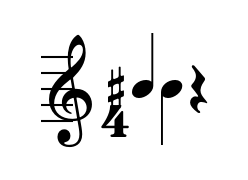
\includegraphics[scale=1]{bravura-example.png}
	\centering
	\caption{Primjer korištenja Bravura fonta}
	\label{fig:bravuraexample}
\end{figure}

U ovom slučaju upotrijebila sam prvu kodnu točku za prikaz notnog crtovlja, kako bih jasnije prikazala pozicioniranje ostalih elemenata. Međutim, u implementaciji aplikacije crtovlje sam ručno "nacrtala", jer generiranje crtovlja korištenjem Bravura fonta nije praktično i ne preporuča se u praksi, s obzirom na to da je širine samo jednog elementa, kao što se vidi na prethodnoj slici.

Simboli su vertikalno pozicionirani tako da se svi centriraju oko treće linije crtovlja. Međutim, note imaju različite tonove i time se trebaju moći vertikalno pomicati po crtovlju. Zbog toga Bravura font nudi naprednu podršku za OpenType ligature koje omogućuju vertikalno pozicioniranje simbola. Ligature su vrsta zamjene znaka u fontu, gdje se dvije ili više kodnih točaka zamjenjuju jednim simbolom. U Bravura fontu se koriste tako što se prvo unese kodna točka koja određuje željenu promjenu vertikalnog položaja, a zatim kodnu točku za sam simbol koji se želi pozicionirati.

Nažalost, nakon puno istraživanja, zbog ograničenja JavaFX biblioteke, nisam uspjela omogućiti korištenje ligatura u svojoj aplikaciji, pa sam sva vertikalna pozicioniranja radila ručno.


%---------------------------- Implementation section ----------------------

\chapter{Implementacija programa}
Za razvoj ove aplikacije koristila sam arhitektonski obrazac (engl. \textit{architectural pattern}) MVC (Model-View-Controller). On razdvaja aplikaciju na tri komponente: model, koji definira i upravlja podacima, pogled (engl. \textit{view}), koji prikazuje podatke korisniku i kontroler (engl. \textit{controller}), koji posreduje između modela i pogleda, definira logiku, te omogućuje interakciju korisnika s aplikacijom. Ovaj obrazac poboljšava organizaciju koda te omogućuje lakše održavanje i testiranje aplikacija.

Korisničko sučelje dizajnirala sam na engleskom jeziku kako bih aplikaciju učinila pristupačnijom široj publici. Za pomoć pri odabiru palete boja koristila sam web alat \textit{Coolors}\footnote{https://coolors.co/}. Sve ikone korištene u dizajnu aplikacije slobodne su za upotrebu u privatne i komercijalne svrhe.

U ovom poglavlju detaljno ću objasniti funkcioniranje svakog dijela aplikacije i prikazati sve zaslone. Poglavlje sam strukturirala prema zaslonima aplikacije, kako bih detaljnije objasnila sve komponente i njihove uloge. Zaslon s glavnom logikom aplikacije, objašnjen u odjeljku \ref{sec:mainscreen}, razradit ću kroz pododjeljke radi bolje jasnoće.

\section{Početni zaslon}
Kada se aplikacija pokrene, prikaže se početni zaslon, koji se može vidjeti na slici \ref{fig:titlescreen}. Ovaj zaslon je jednostavan i sastoji se od naslova, te tri gumba. Pritiskom na prvi gumb otvara se zaslon za odabir datoteke s pjesmom s računala, što je detaljnije objašnjeno u odjeljku \ref{sec:uploadscreen}. Drugi gumb otvara zaslon s izborom pjesama iz male knjižnice koju sam pripremila, a koji je detaljno objašnjen u odjeljku \ref{sec:libraryscreen}. Treći gumb vodi na zaslon s postavkama klavijature, o kojem je više riječi u odjeljku \ref{sec:settingsscreen}.

\begin{figure}[h]
	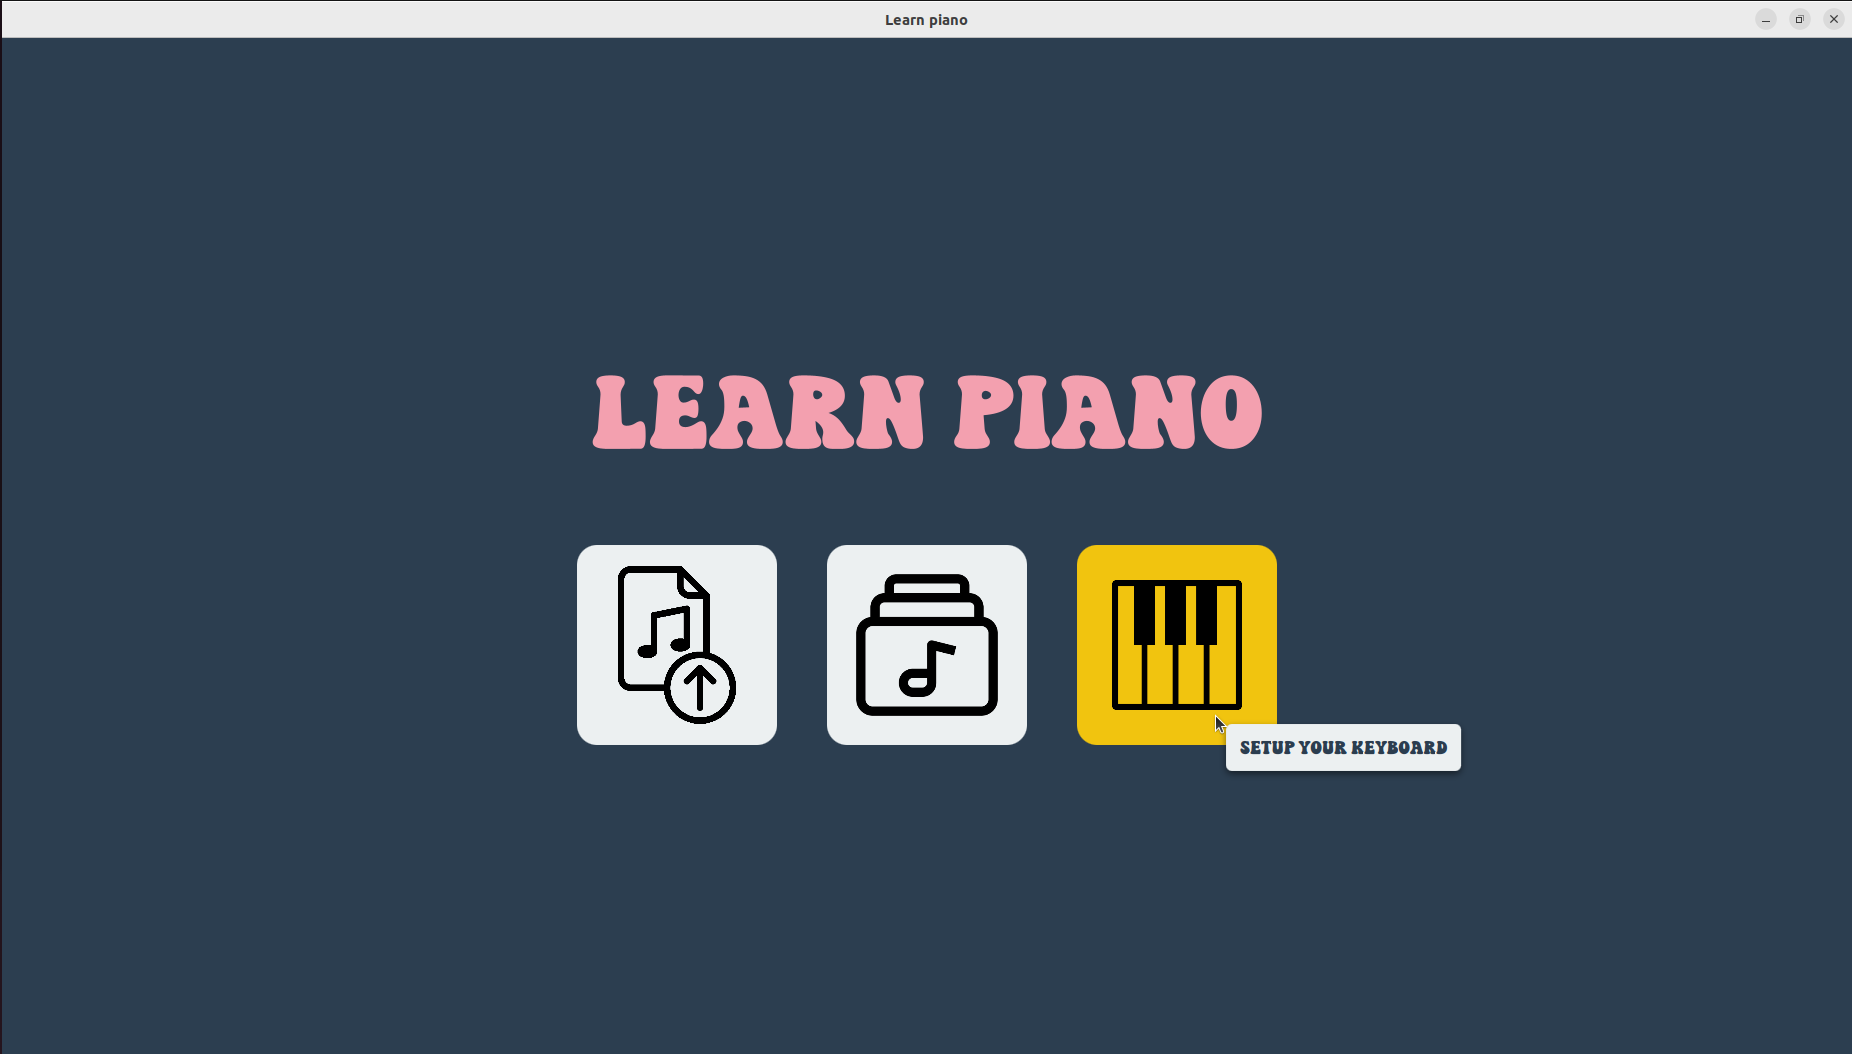
\includegraphics[width=\textwidth]{title-screen.png}
	\centering
	\caption{Početni zaslon aplikacije}
	\label{fig:titlescreen}
\end{figure}

Prelaskom kursora preko gumba, pozadina se mijenja u žutu kako bi se jasno istaknuo mogući odabir. Umjesto teksta, odlučila sam koristiti ikone za označavanje gumba, što poboljšava vizualni dizajn, ali može smanjiti jasnoću. Zbog toga sam dodala opisne oznake (engl. \textit{tooltip}) koje se prikazuju kada se kursor nalazi iznad gumba. Mijenjanje pozadine gumba u žutu boju i dodavanje opisnih oznaka na gumbe s ikonama konzistentno je primijenjeno u cijeloj aplikaciji.

\subsection{Navigacija aplikacijom}
Kako bih si olakšala navigaciju među različitim zaslonima, implementirala sam \textit{NavigationController} koji preuzima svu logiku navigacije. Ovaj kontroler je implementiran koristeći oblikovni obrazac (engl. \textit{design pattern}) \textit{singleton}. Za njega i sve ostale \textit{singleton} objekte u aplikaciji koristila sam enumeraciju (engl. \textit{enum}) s jednom vrijednošću (engl. \textit{case}) pod nazivom \textit{INSTANCE}. Time sam osigurala jednostavan pristup kontroleru iz bilo kojeg dijela aplikacije gdje je potreban.

\textit{NavigationController} interno pohranjuje stog (engl. \textit{stack}) drugih kontrolera odgovornih za upravljanje zaslonima. Svi oni implementiraju sučelje \textit{BaseViewController}, koje zahtijeva implementaciju metode \textit{Pane getView()}, koja vraća pogled kojim taj kontroler upravlja. \textit{NavigationController} nudi tri jednostavne metode za upravljanje navigacijom, navedene u nastavku, kao i metodu \textit{Stage getStage()} koja omogućuje dohvat objekta \textit{Stage} iz bilo kojeg dijela aplikacije.

\begin{lstlisting}
void init(Stage stage, BaseViewController viewController);
void push(BaseViewController viewController);
void pop();
\end{lstlisting}

Prva metoda koristi se za inicijalizaciju navigacije početnim \textit{stage-om} i kontrolerom, u mojem slučaju \textit{TitleViewController-om} koji upravlja početnim zaslonom. Metoda \textit{push} dodaje predani kontroler na interni stog i prikazuje njegov pogled. Slično tome, metoda \textit{pop} uklanja posljednji kontroler sa stoga i prikazuje pogled kontrolera koji se nalazi neposredno ispod njega, vraćajući aplikaciju na prethodni zaslon.

\section{Zaslon za odabir pjesme s računala}
\label{sec:uploadscreen}
Odabirom lijevog gumba na početnom zaslonu otvara se zaslon za odabir pjesme s računala, prikazan na slici \ref{fig:uploadscreen}. Klikom na gumb \textit{Choose a file} otvara se datotečni izbornik u kojemu se mogu odabrati datoteke s nastavcima \textit{.xml} i \textit{.musicxml}. U gornjem lijevom kutu zaslona smješten je gumb sa ikonom strelice, koji omogućava povratak na prethodni zaslon. Ovaj gumb prisutan je na svakom zaslonu osim na početnom.

\begin{figure}[h]
	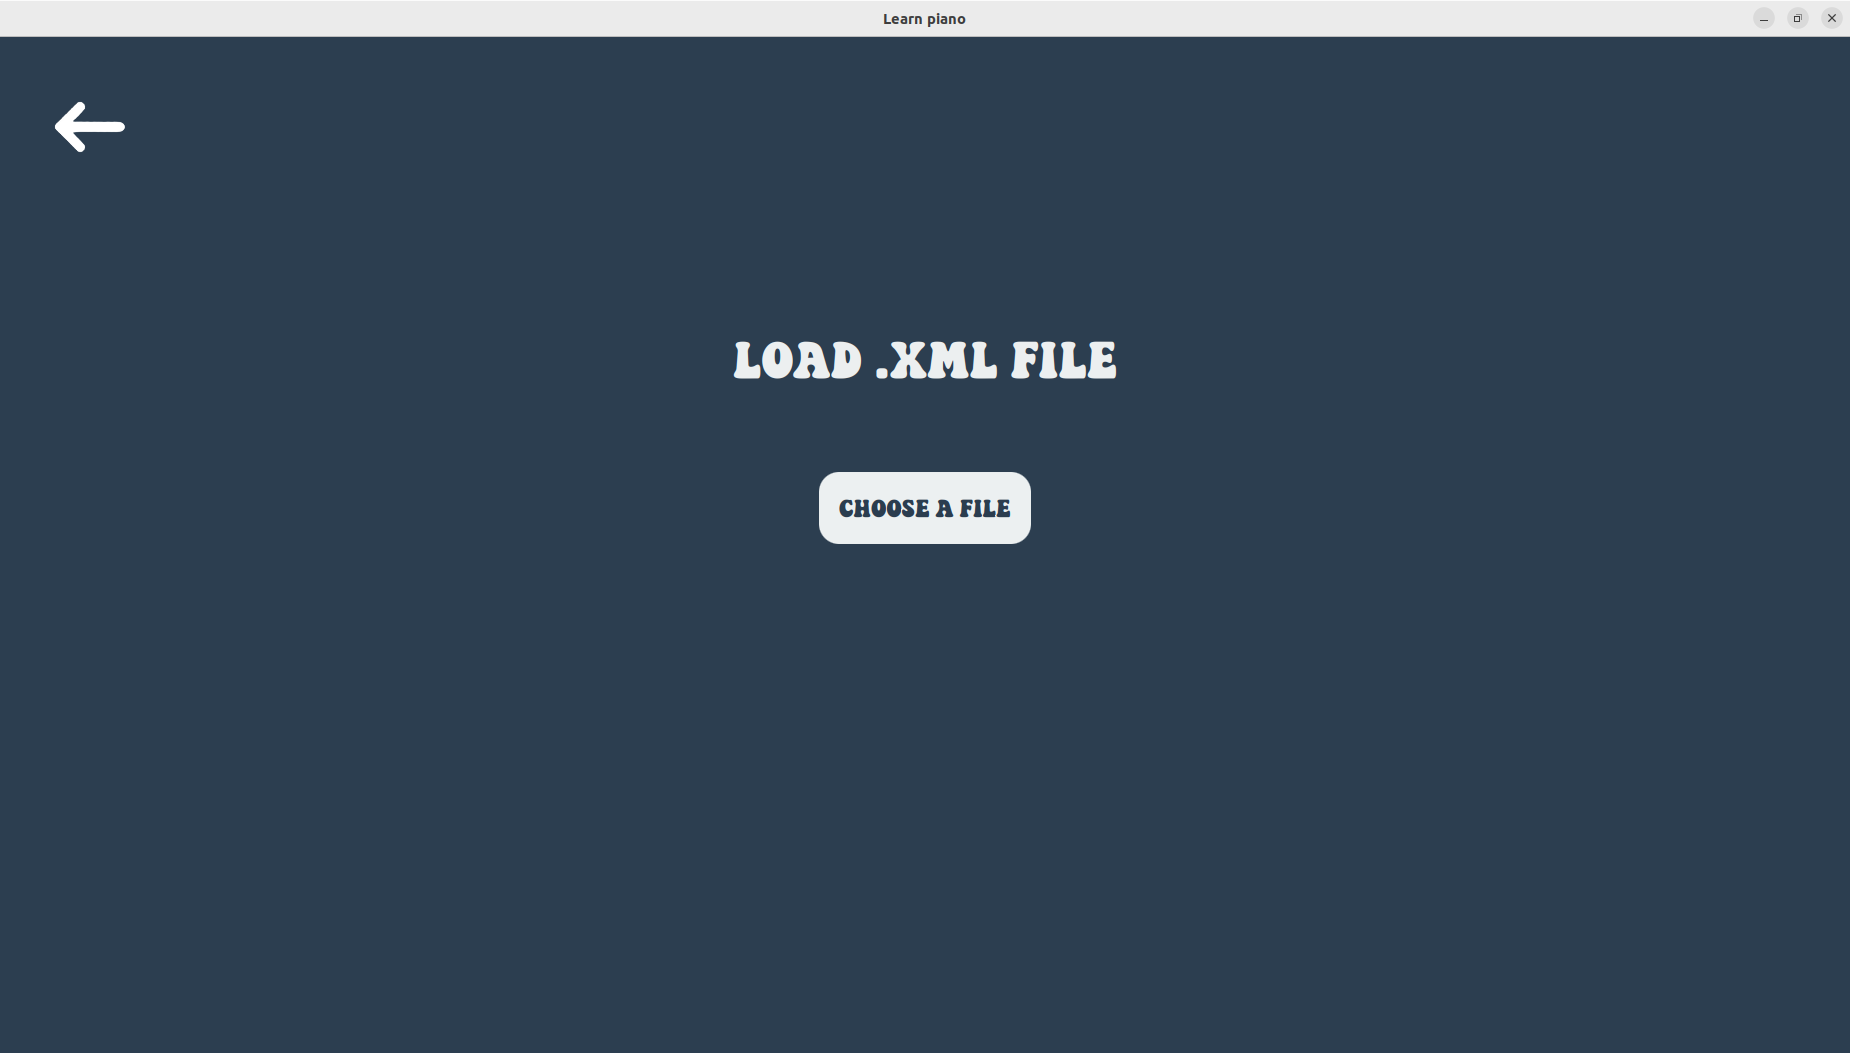
\includegraphics[width=\textwidth]{upload-screen.png}
	\centering
	\caption{Zaslon za odabir pjesme s računala}
	\label{fig:uploadscreen}
\end{figure}

U slučaju da odabrana datoteka odgovara formatu koji moja aplikacija podržava, prikazuje se zaslon kao na slici \ref{fig:uploadconfirm}. Na zaslonu se prikazuje naziv odabrane datoteke te su dostupna dva gumba. Klikom na gumb \textit{Confirm}, potvrđuje se odabir datoteke i otvara se glavni zaslon aplikacije. Gumb \textit{Load another file} omogućuje ponovno otvaranje datotečnog izbornika za odabir druge datoteke.

\begin{figure}[h]
	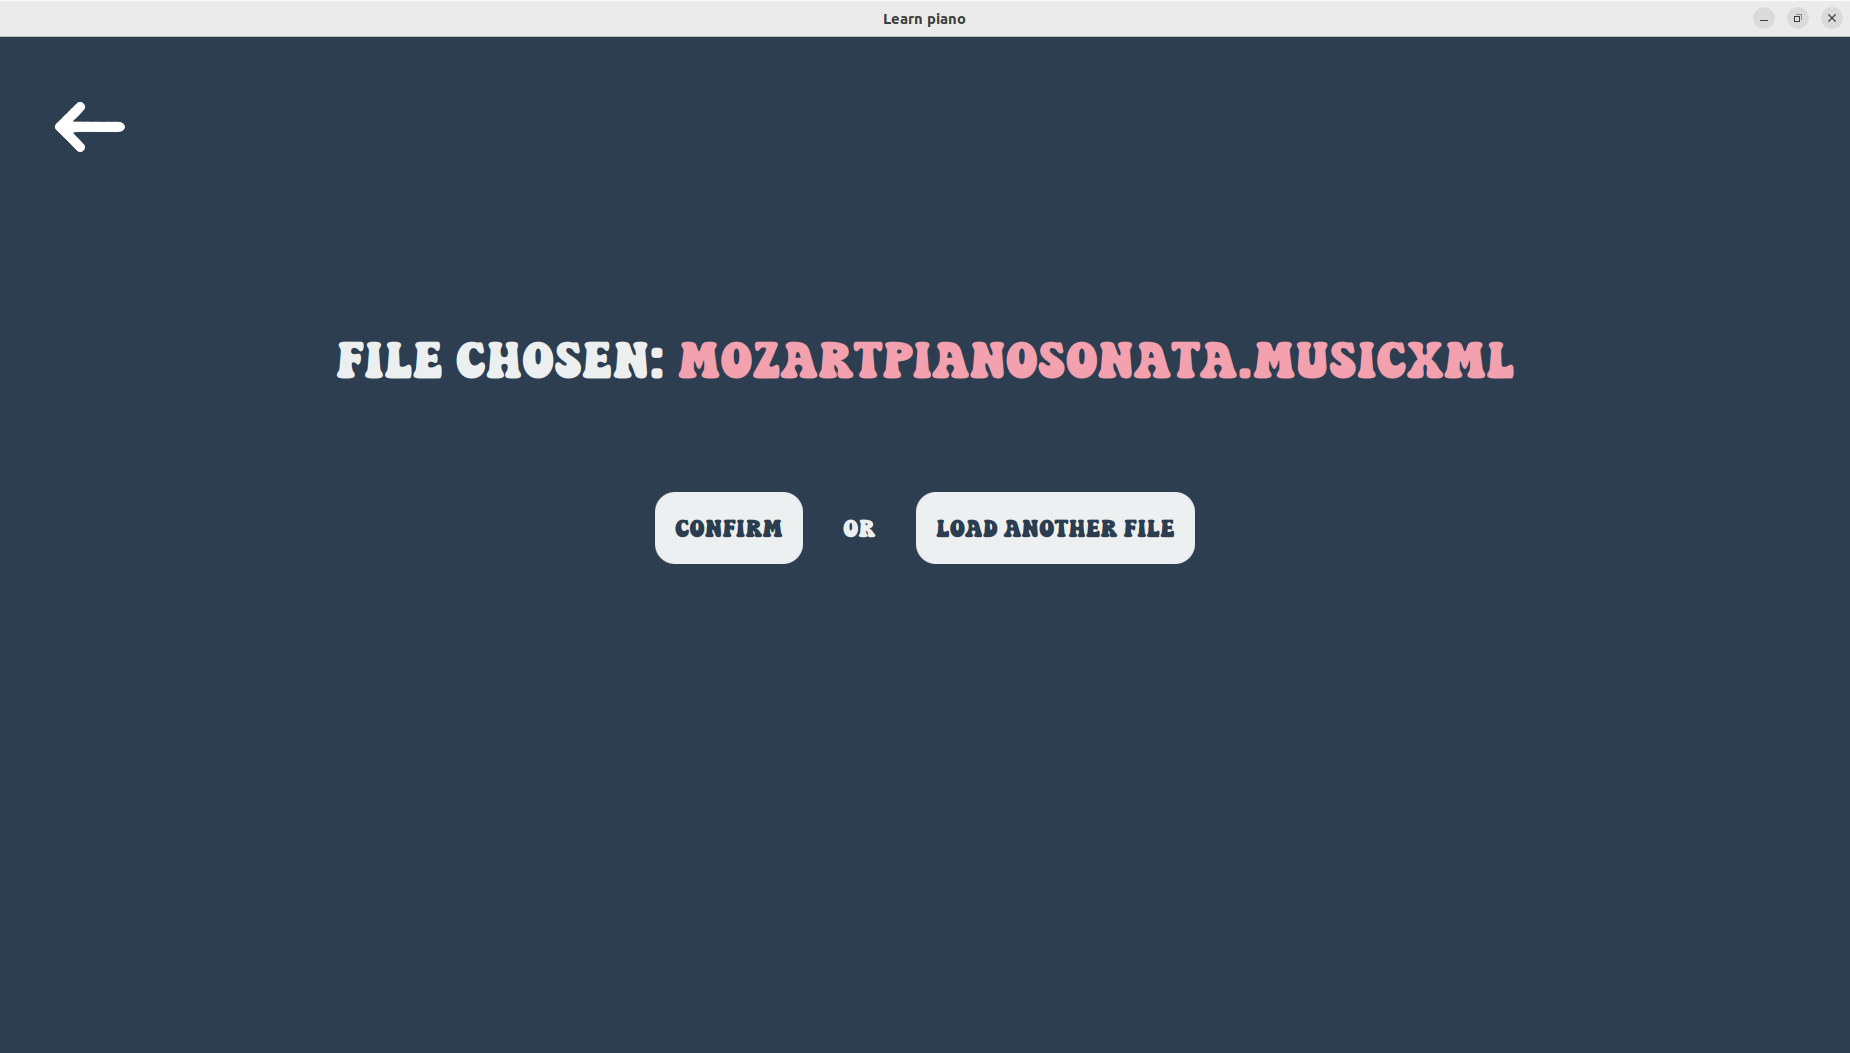
\includegraphics[width=\textwidth]{upload-confirm.png}
	\centering
	\caption{Zaslon za potvrdu pjesme}
	\label{fig:uploadconfirm}
\end{figure}

\subsection{Podržani i nepodržani formati}
\label{sec:formats}
Ako format odabrane datoteke nije podržan u aplikaciji, na zaslonu se prikazuje pogreška, što je vidljivo na slici \ref{fig:uploaderror}. Mogu se pojaviti tri različite vrste pogrešaka. Prva se javlja ako datoteka nije uopće u MusicXML formatu ili ako njezin korijenski element nije \textit{<score-partwise>}. Iako datotečni sustav filtrira datoteke u formatima \textit{.musicxml} i \textit{.xml}, format \textit{.xml} može sadržavati razne vrste datoteka, pa postoji mogućnost da korisnik odabere datoteku koja nije u MusicXML formatu.

\begin{figure}[h]
	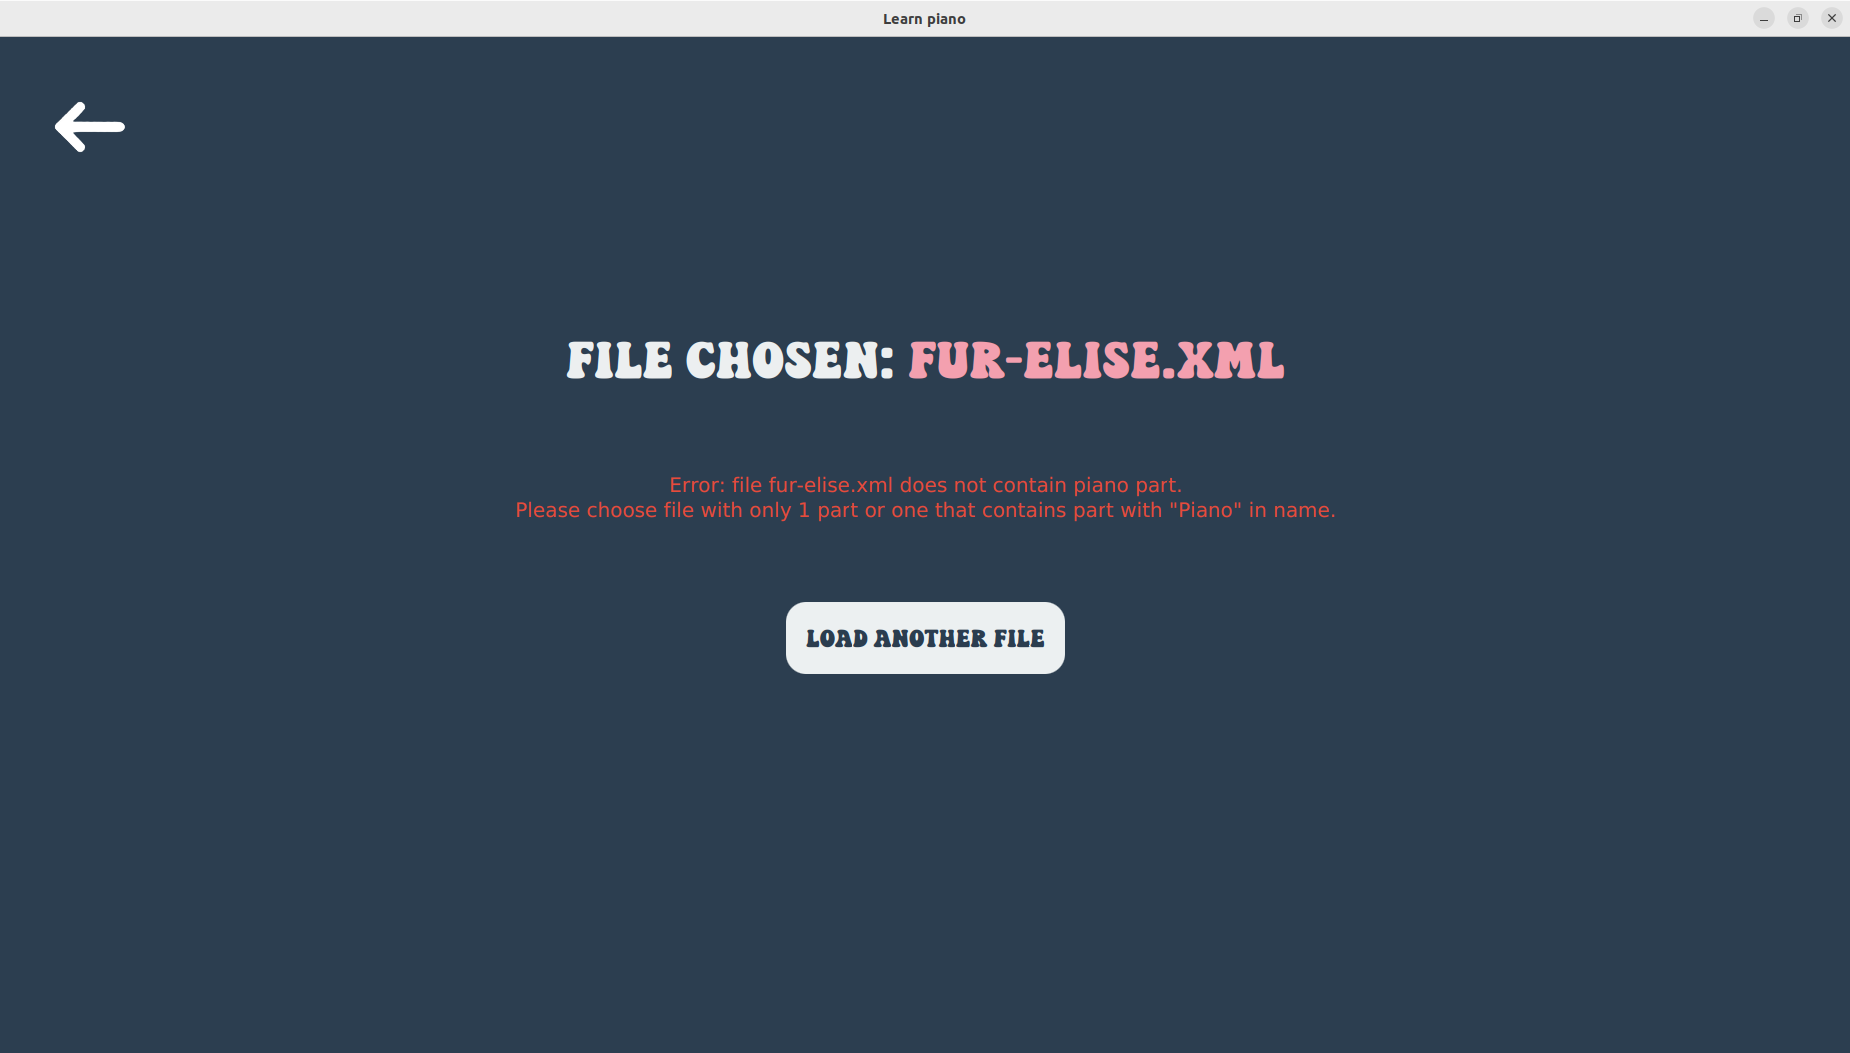
\includegraphics[width=\textwidth]{upload-error.png}
	\centering
	\caption{Zaslon za odabir pjesme sa pogreškom}
	\label{fig:uploaderror}
\end{figure}

MusicXML datoteke mogu biti organizirane na dva različita načina, ovisno o korijenskom elementu. Element \textit{<score-partwise>} strukturira notni zapis prema dijelovima (engl. \textit{part}), poput različitih instrumenata ili vokalnih linija. Unutar svakog dijela, zapisi su organizirani po taktovima. Ovaj format je najčešći i najintuitivniji za većinu korisnika, jer slijedi tradicionalnu organizaciju partitura. S druge strane, \textit{<score-timewise>} strukturira notni zapis prema taktovima. Svaki takt sadrži informaciju za sve dijelove u tom taktu. Ovaj format je koristan za obradu glazbenih podataka gdje je važno imati pristup informacijama prema vremenskoj liniji.

U nastavku je prikazana metoda koja deserijalizira odabranu datoteku u \textit{ScorePartwise} objekt koristeći biblioteku \textit{ProxyMusic}. Ona se nalazi u razredu \textit{XMLConverter} koji je implementiran kao \textit{singleton} objekt kroz enumeraciju, kako bi deserijalizirani \textit{ScorePartwise} objekt mogao biti dostupan u bilo kojem dijelu aplikacije. Ako dođe do iznimke (npr. datoteka nije u ispravnom formatu, deserijalizacija ne uspije ili dođe do problema s ulazno-izlaznim operacijama), metoda vraća \textit{false} i aplikacija obavještava korisnika o pogrešci.

\begin{lstlisting}
public boolean unmarshall(File file) {
	try (InputStream inputStream = new FileInputStream(file)) {
		Object unmarshalledObject = Objects.requireNonNull(Marshalling.unmarshal(inputStream));
		score = (ScorePartwise) unmarshalledObject;
		return true;
	} catch (Marshalling.UnmarshallingException | ClassCastException | NullPointerException | IOException e) {
		return false;
	}
}
\end{lstlisting}

Druga kontrola koju aplikacija provodi odnosi se na prisutnost klavirskog dijela u datoteci. Budući da su datoteke formata \textit{<score-partwise>} organizirane po dijelovima, na početku se nalazi obavezan element \textit{<part-list>} koji sadrži popis svih dijelova skladbe.

Ako datoteka sadrži samo jedan dio, aplikacija automatski pretpostavlja da je taj dio namijenjen klaviru, budući da nema drugih kriterija za identifikaciju. Međutim, ako datoteka sadrži više dijelova (npr. dodatni instrument ili vokalnu liniju), aplikacija pretražuje imena dijelova kako bi provjerila sadrži li neki od njih riječ "Piano" te ako ga pronađe, taj dio smatra klavirskim. U slučaju da aplikacija ne uspije pronaći dio za klavir, korisniku će prikazati poruku o pogrešci, kao što je prikazano na slici \ref{fig:uploaderror}.

Treća i posljednja provjera odnosi se na broj crtovlja (engl. \textit{staff}) u dijelu. Prvi takt svakog dijela sadrži element \textit{<attributes>}, koji pruža ključne informacije o pjesmi, poput ljestvice, vremenske oznake, ključeva, te elementa \textit{<staves>}. Ovaj element sadrži broj koji označava koliko crtovlja pjesma ima. U slučaju da taj element nije prisutan, pretpostavlja se da pjesma ima jedno crtovlje.

Aplikacija podržava prikaz jednog ili dva crtovlja. Ako pjesma ima jedno crtovlje, ono je namijenjeno desnoj ruci. Ako ima dva crtovlja, prvo je za desnu ruku, a drugo za lijevu. U slučaju da \textit{<attributes>} element nije pronađen ili broj crtovlja prelazi dva, aplikacija prikazuje odgovarajuću poruku o pogrešci na ekranu.

Uz pogrešku, na ekranu je također prikazan naziv odabrane datoteke te gumb \textit{Load another file} kojim se putem datotečnog izbornika može odabrati druga datoteka.

\section{Zaslon za odabir pjesme iz knjižnice}
\label{sec:libraryscreen}
Odabirom srednjeg gumba na početnom zaslonu otvara se zaslon za odabir pjesme iz knjižnice, koji je prikazan na slici \ref{fig:libraryscreen}. Iako je prvotna ideja aplikacije bila da korisnik učita datoteku sa željenom pjesmom, odlučila sam implementirati i malu knjižnicu s nekoliko unaprijed ponuđenih pjesama. Idealno ova knjižnica sadržavala bi puno veći broj pjesama, ali to bi zahtijevalo značajan trud u pronalaženju i pripremi velikog broja datoteka, što nadilazi opseg ovog rada. Ipak, knjižnica služi kao dokaz koncepta i olakšava testiranje funkcionalnosti aplikacije.

\begin{figure}[h]
	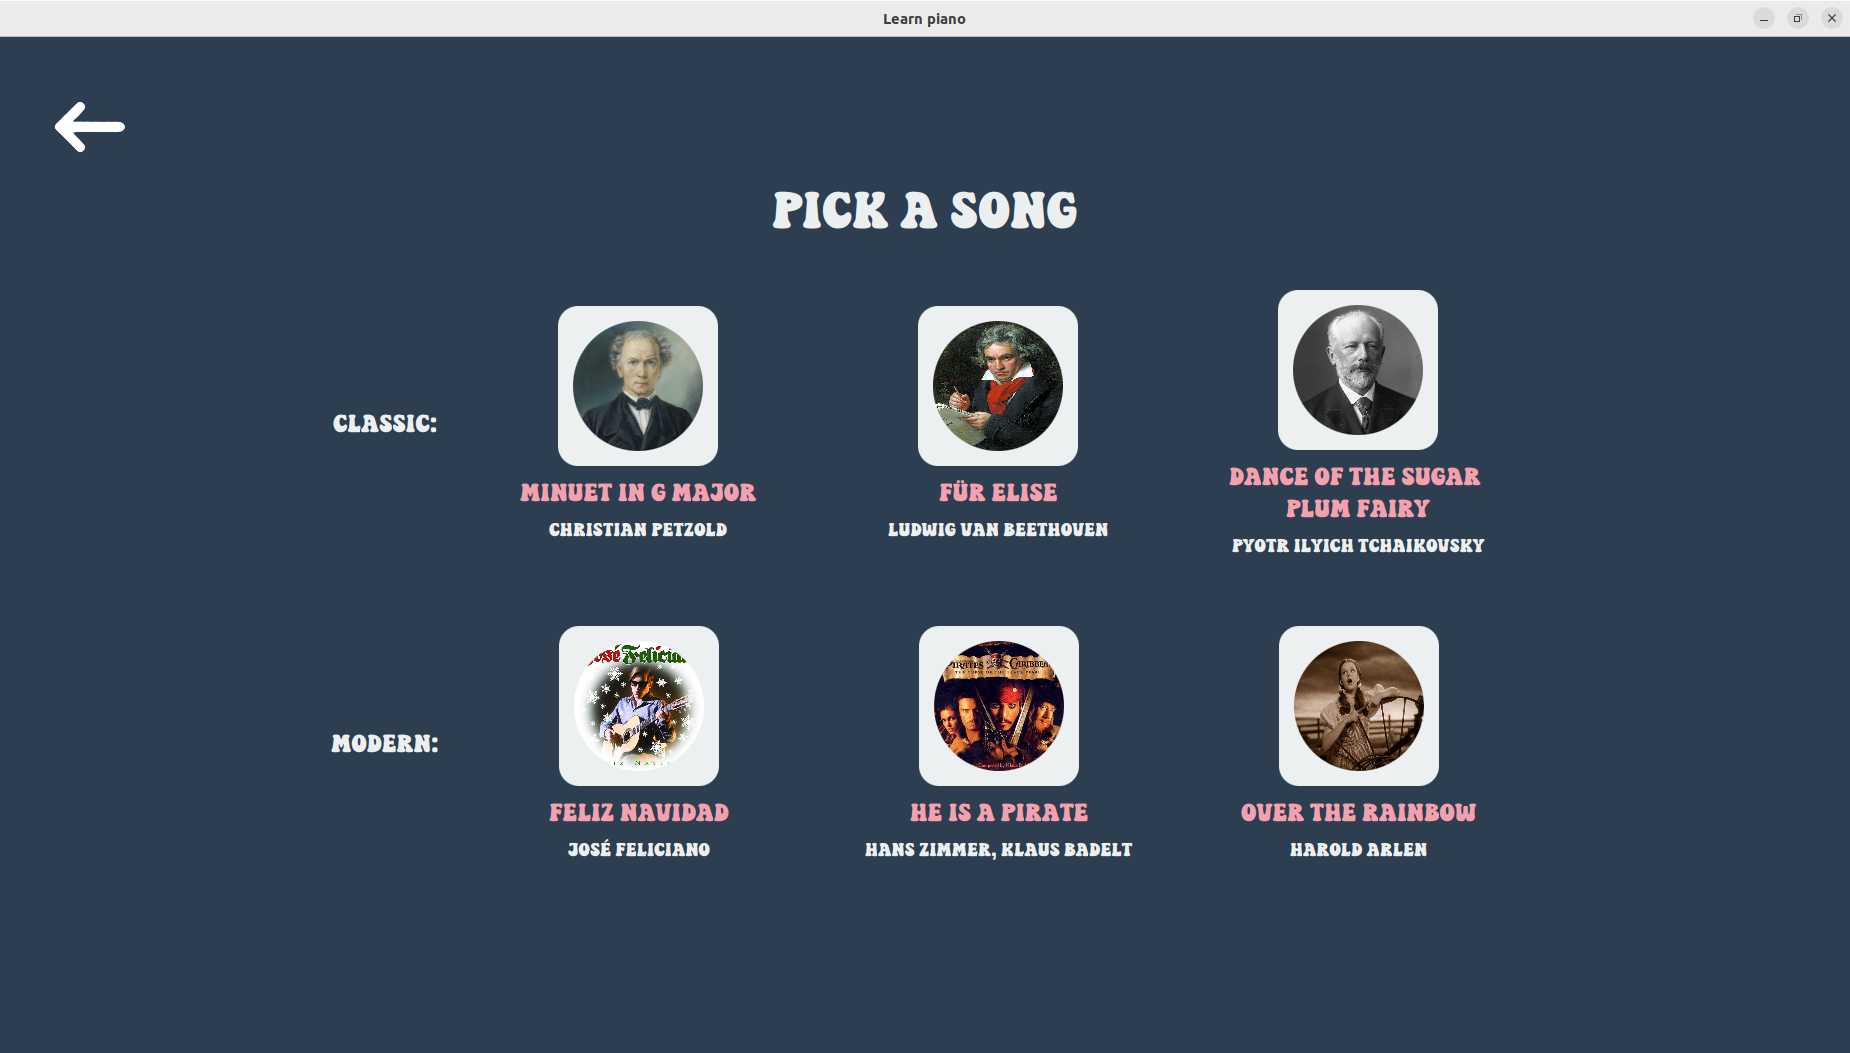
\includegraphics[width=\textwidth]{library-screen.png}
	\centering
	\caption{Zaslon za odabir pjesme iz knjižnice}
	\label{fig:libraryscreen}
\end{figure}

Odlučila sam u knjižnicu dodati tri klasične skladbe i tri moderne pjesme. Pjesme su različitih težina gdje je prva u oba žanra najjednostavnija za sviranje, a zadnja najteža. Za svaku pjesmu navedeni su naziv, ime umjetnika (skladatelja/izvođača/pjevača), te fotografija umjetnika, koja služi kao gumb za odabir te pjesme. Odabirom pjesme klikom na fotografiju, odgovarajuća datoteka se učitava iz resursa aplikacije i deserijalizira na način opisan u odjeljku \ref{sec:formats}, te se otvara glavni zaslon aplikacije. Za ove datoteke nije potrebno provoditi dodatne provjere, budući da su već unaprijed provjerene i sigurno ispravne.

Pjesme odnosno skladbe koje sam odabrala su redom: "Menuet u G duru" skladatelja Christiana Petzolda, "Za Elizu" skladatelja Ludwiga van Beethovena, "Ples šećerne vile" skladatelja Petra Iljiča Čajkovskog, "Feliz Navidad" pjevača i tekstopisca Joséa Feliciana, "He is a pirate" skladatelja Klausa Badelta i Hansa Zimmera za film "Pirati s Kariba: Prokletstvo Crnog bisera" i zadnja "Over the rainbow" skladatelja Harolda Arena za film "Čarobnjak iz Oza". Sve skladbe preuzete su sa stranice MuseScore\cite{musescore}.

\section{Zaslon za postavke klavijature}
\label{sec:settingsscreen}
Odabirom desnog gumba na početnom zaslonu otvara se zaslon za odabir klavijature i postavljanje njenog raspona, koji je prikazan na slici \ref{fig:keyboardsetupscreen}. Na ovome zaslonu korisnik može odabrati spojenu klavijaturu iz padajućeg izbornika koji prikazuje sve dostupne MIDI uređaje. Java nativno podržava rad s MIDI uređajima i protokolom putem paketa \textit{javax.sound.midi}. Desno od padajućeg izbornika nalazi se gumb za osvježavanje liste dostupnih uređaja. Zadani odabir je posljednji uređaj na listi, budući da sam na temelju testiranja ustanovila da je to obično uređaj koji je fizički spojen na računalo. Prije njega nalaze se MIDI uređaji koji su aplikacijski ili virtualni, odnosno već ugrađeni u operacijski sustav. Promjenom odabira uređaja u padajućem izborniku, mijenja se uređaj u aplikaciji i taj proces je detaljnije objašnjen u pododjeljku \ref{sec:mididevices}.

\begin{figure}[h]
	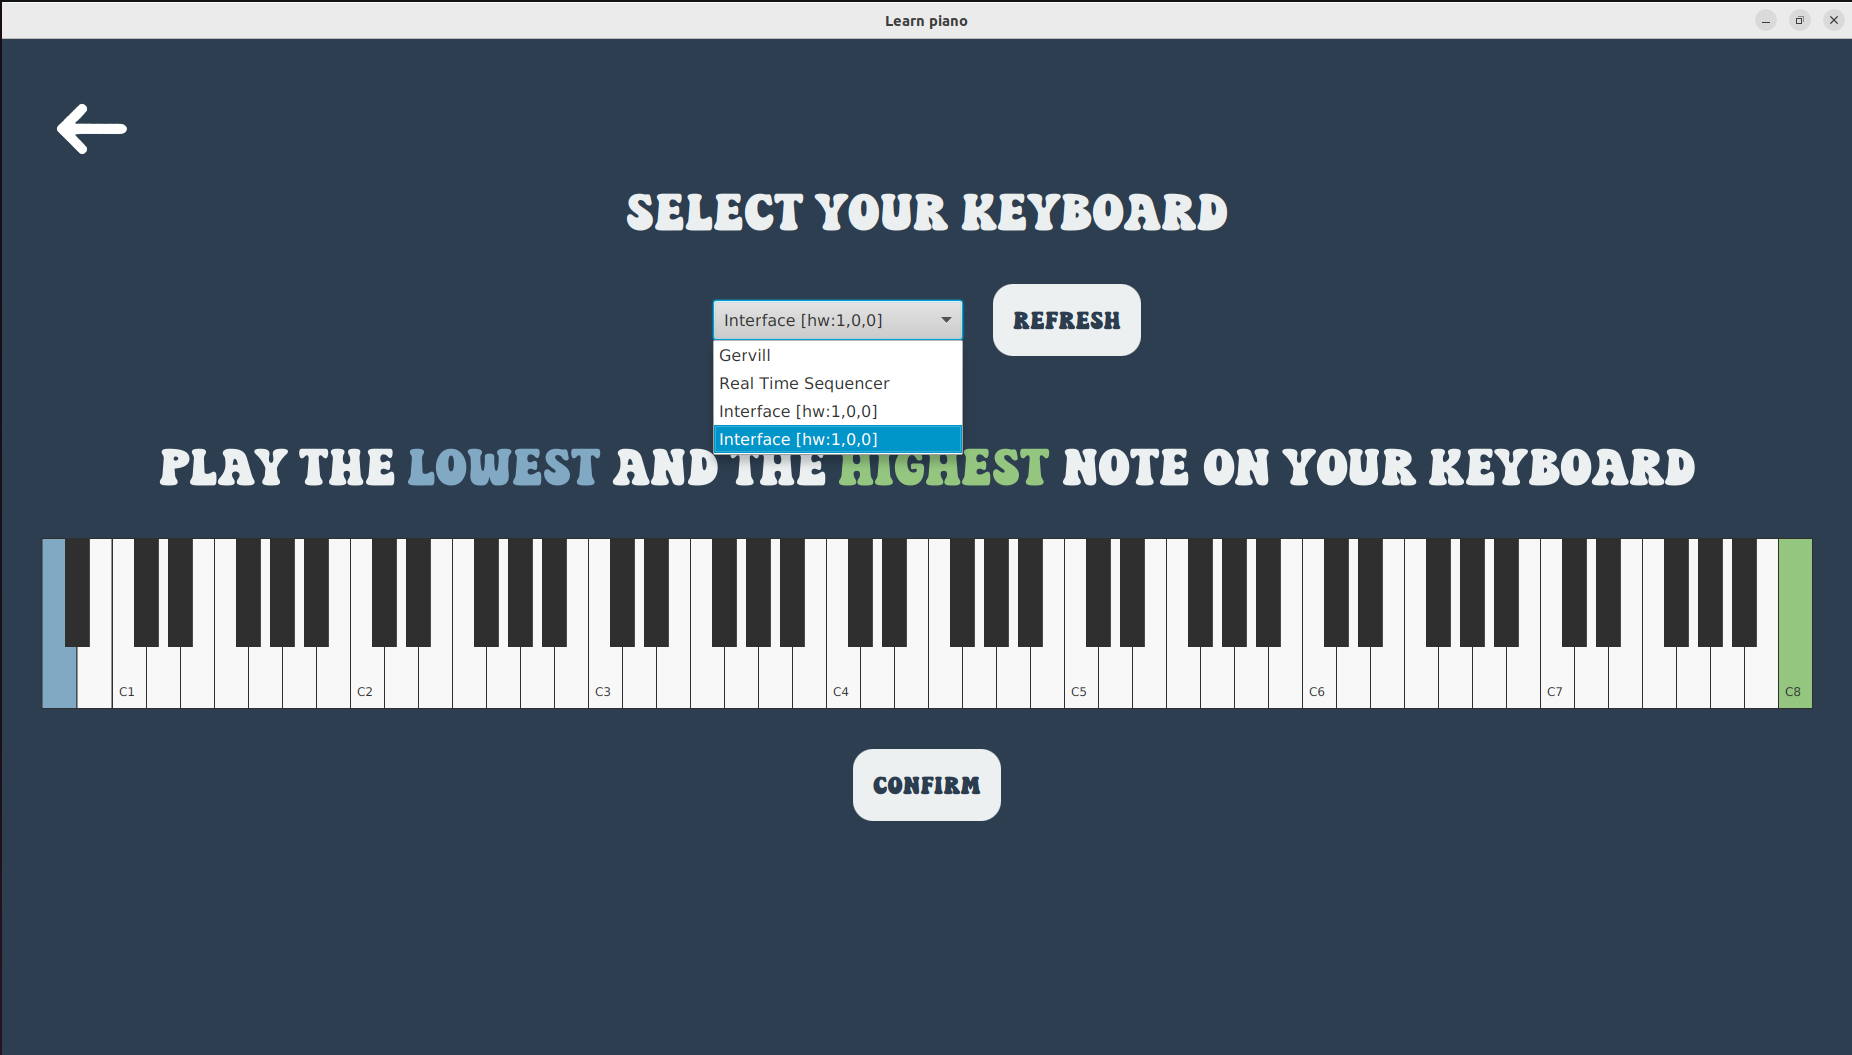
\includegraphics[width=\textwidth]{keyboard-setup-screen.png}
	\centering
	\caption{Zaslon za postavke klavijature}
	\label{fig:keyboardsetupscreen}
\end{figure}

Ispod izbornika za odabir MIDI uređaja nalazi se uputa za korisnika da odsvira najnižu i najvišu notu na svojoj klavijaturi. To je važno jer nisu sve klavijature punog opsega koncertnog klavira (A0 - C8), što znači da neke vrlo niske ili visoke tonove na njima nije moguće odsvirati. Ovo može predstavljati problem kod načina sviranja koji čeka da korisnik odsvira točnu notu, jer ju on možda neće moći odsvirati.

Na slici \ref{fig:keyboardsetuprange} prikazan je rezultat odabira raspona, pri čemu je plavom bojom označena najniža nota, a zelenom najviša. Kada korisnik pritisne tipku na klavijaturi i ako je ona različita od prethodno pritisnute, ažurira se raspon nota tako da nova i prethodna tipka definiraju najnižu i najvišu notu. Zaslon se zatim osvježava kako bi prikazao te promjene, dinamički prilagođavajući plavu i zelenu oznaku prema korisnikovom odabiru.

\begin{figure}[h]
	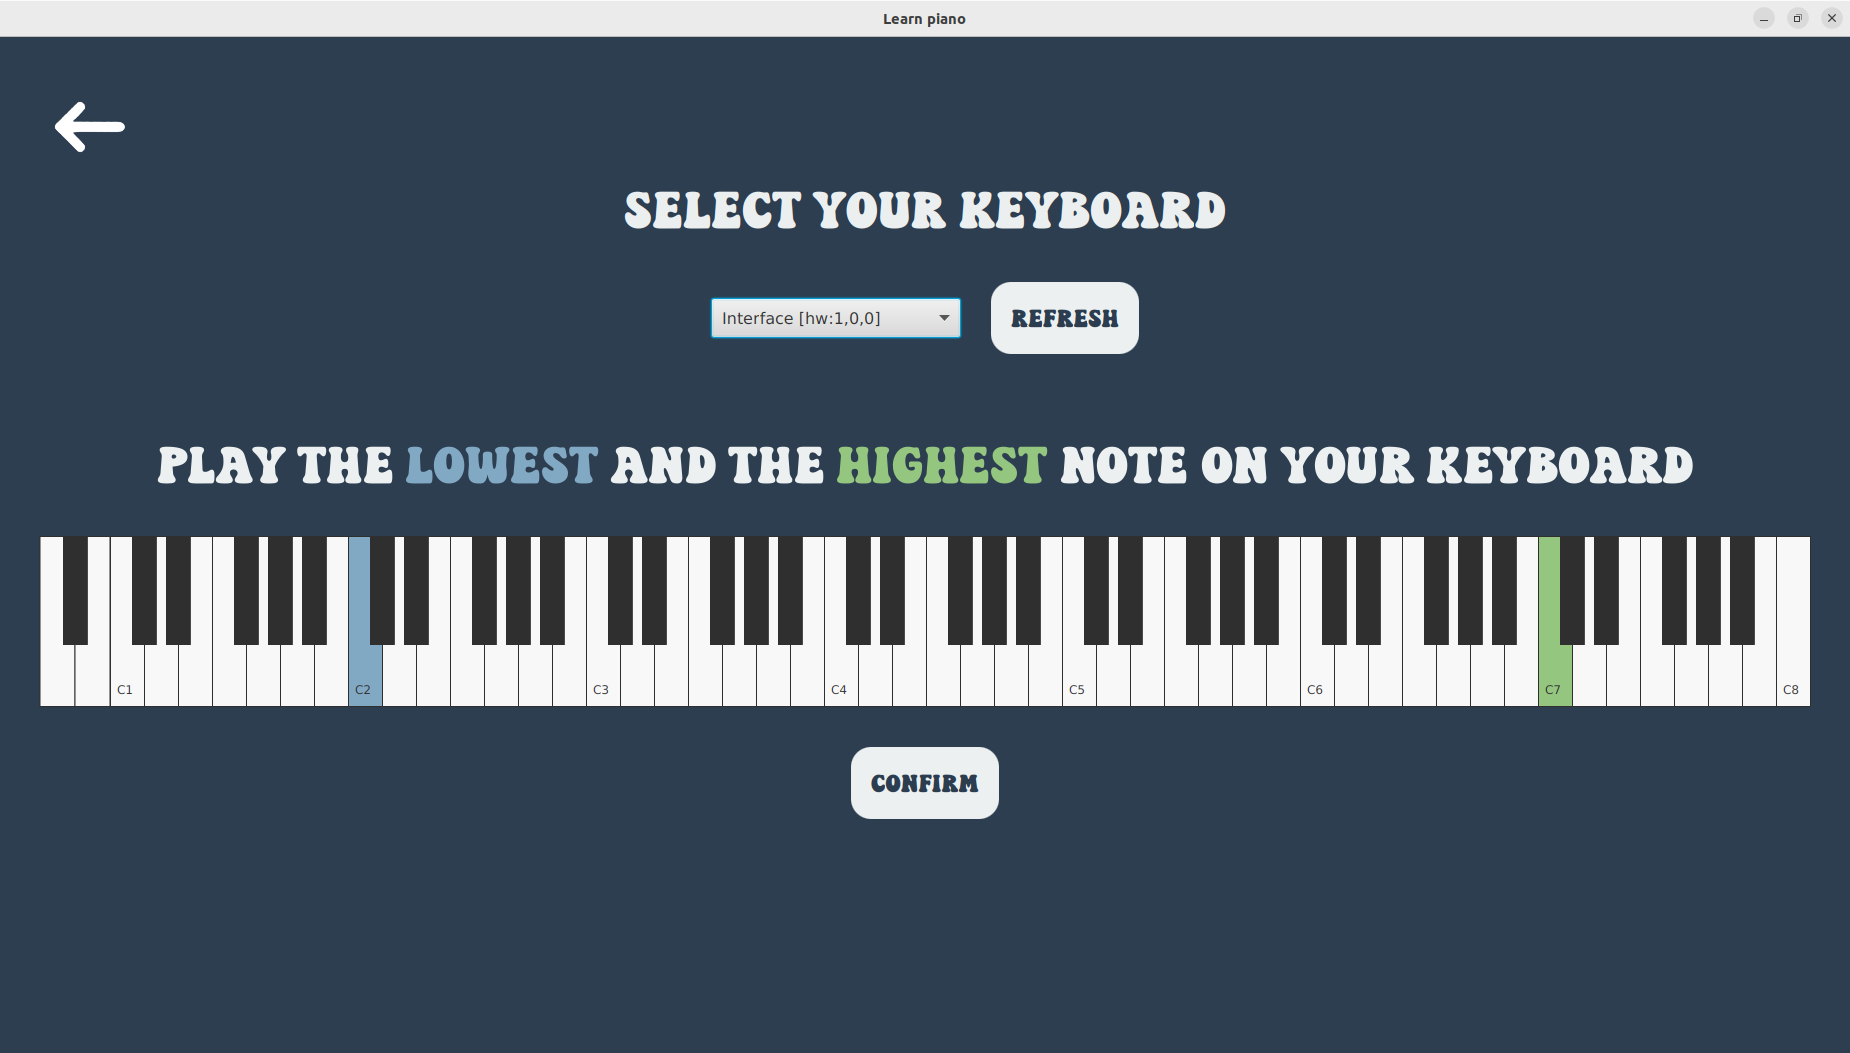
\includegraphics[width=\textwidth]{keyboard-setup-range.png}
	\centering
	\caption{Zaslon za postavke klavijature s odabranim rasponom}
	\label{fig:keyboardsetuprange}
\end{figure}

Klikom na gumb \textit{Confirm} sprema se korisnikov odabir raspona klavijature, nakon čega se aplikacija vraća na prethodni, odnosno početni zaslon. Također, korisnik se može vratiti na prethodni zaslon pritiskom na strelicu za povratak u gornjem lijevom kutu, ali u tom slučaju korisnikov odabir raspona klavijature neće biti spremljen. Postavljanje ovih postavki nije obavezno, jer će aplikacija u većini slučajeva ispravno funkcionirati i sa zadanim postavkama: posljednji uređaj na listi biti će automatski odabran, a raspon klavijature postavljen na standardni koncertni klavir.

\subsection{Upravljanje MIDI uređajima}
\label{sec:mididevices}
Za upravljanje MIDI uređajima unutar aplikacije napisala sam razred \textit{MidiDeviceManager}, koji je također implementiran kao \textit{singleton} objekt, osiguravajući da postoji samo jedna instanca razreda tijekom rada aplikacije. Ovaj razred omogućuje centralizirano upravljanje MIDI uređajima, uključujući povezivanje, postavljanje i zatvaranje uređaja kroz sljedeće metode:

\begin{lstlisting}
List<MidiDevice.Info> getDeviceInfos();
MidiDevice.Info getChosenDeviceInfo();
void setDevice(MidiDevice.Info deviceInfo);
MidiInputReceiver getReceiver();
void close();
\end{lstlisting}

Metoda \textit{getDeviceInfos} vraća listu informacija svih dostupnih MIDI uređaja koje sustav prepoznaje, a to se može napraviti ovako: \lstinline|MidiSystem.getMidiDeviceInfo()|. Metoda \textit{getChosenDeviceInfo} vraća informacije o trenutno odabranom uređaju. Ako nijedan uređaj nije odabran, ili se odabrani uređaj više ne nalazi u listi dostupnih uređaja, automatski se odabire posljednji uređaj s liste dostupnih, što odgovara zadanom ponašanju prethodno opisanim u tekstu.

Postavljanje korisnikovog odabira postiže se koristeći metodu \textit{setDevice}, koja postavlja i otvara odabrani MIDI uređaj na temelju predanih informacija. U slučaju da već postoji otvoreni uređaj, on se zatvara prije otvaranja novog. Otvaranje uređaja provodi se na način naveden u nastavku. Nakon što se dohvati i otvori željeni uređaj, postavlja se prijemnik (engl. \textit{receiver}), za predajnik (engl. \textit{transmitter}) uređaja.

\begin{lstlisting}
try {
	assert chosenDeviceInfo != null;
	currentDevice = MidiSystem.getMidiDevice(chosenDeviceInfo);
	currentDevice.open();
	
	Transmitter transmitter = currentDevice.getTransmitter();
	transmitter.setReceiver(receiver);
} catch (MidiUnavailableException | NullPointerException ignored) {
}
\end{lstlisting}

Metoda \textit{getReceiver} dohvaća prijemnik, a ako on nije već postavljen, inicijalizira MIDI uređaj na zadane postavke. Prijemnik se implementira kroz sučelje \textit{Receiver}, što sam to napravila u razredu \textit{MidiInputReceiver}. Detaljnija implementacija ovog sučelja može se pronaći u pododjeljku \ref{sec:midimessages}.

Na kraju, metoda \textit{close} omogućuje zatvaranje trenutno otvorenog MIDI uređaja, ako je otvoren, čime se osigurava pravilno upravljanje resursima kod gašenja aplikacije.

Osim metoda za rad s MIDI uređajima, ovaj razred pruža i pristup modelu klavijature putem metode \textit{getKeyboardModel}. Ako model klavijature još nije definiran, automatski se kreira novi model s rasponom koncertnog klavira. Metoda \textit{setKeyboardModel} omogućuje postavljanje novog modela klavijature.

\subsection{Obrada MIDI poruka}
\label{sec:midimessages}
Razred \textit{MidiInputReciver} predstavlja implementaciju sučelja \textit{Receiver}, zaduženog za primanje i obradu MIDI poruka, specifično onih koje se odnose na pritisak i otpuštanje klavirskih tipki. Ključna metoda koju je potrebno implementirati u ovom razredu je \textit{send}. Ona prima i obrađuje primljene MIDI poruke, a njena implementacija prikazana je u nastavku.

\begin{lstlisting}
@Override
public void send(MidiMessage message, long timeStamp) {
	int status = message.getStatus();
	if (status == 128 || status == 144) {
		byte[] data = message.getMessage();
		int key = data[1] & 0xFF;
		int speed = data[2] & 0xFF;

		if (status == 144 && speed != 0 && keyPressedListener != null) {
			keyPressedListener.onAction(key);
		} else if (keyReleasedListener != null) {
			keyReleasedListener.onAction(key);
		}
	}
}
\end{lstlisting}

Primjer sadržaja MIDI poruke prikazan je na slici \ref{fig:midimessage}. Poruka se obično sastoji od tri bajta: prvi je statusni bajt, koji određuje tip poruke i kanal, dok druga dva bajta sadrže parametre, kao što su vrijednost pritisnute tipke i brzina pritiska. Statusni bajt uvijek započinje s bitom 1, dok podatkovni bajtovi s bitom 0.

\begin{figure}[h]
	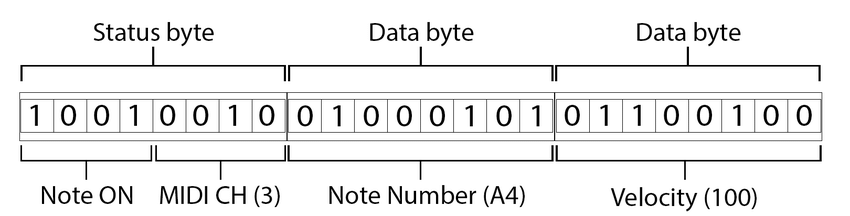
\includegraphics[width=\textwidth]{midi-message.png}
	\centering
	\caption{Primjer MIDI poruke \cite{midimessage}}
	\label{fig:midimessage}
\end{figure}

Metoda \textit{send} prvo provjerava status poruke. Iako postoji više mogućih statusa, za moj rad su ključni status 128, koji označava otpuštanje tipke, i status 144 koji označava pritisak tipke. Zbog pojednostavljenja implementacije, neki modeli klavijatura (uključujući onaj koji koristim) ne koriste status 128 za označavanje otpuštanja tipke. Umjesto toga, koriste kombinaciju statusa 144 s brzinom pritiska postavljenom na 0. Stoga, u mojoj aplikaciji oba ova pristupa prepoznajem kao otpuštanje tipke.

Unutar metode, poruka se raščlanjuje pomoću metode \textit{getMessage}, koja vraća byte polje podataka. Prvi element u tom polju sadrži prethodno dobiven status, dok drugi element \textit{data[1]} sadrži vrijednost pritisnute tipke. Ta vrijednost je u rasponu od 0 do 127, pri čemu klavijature obično koriste interval od 21 do 108: vrijednost 21 označava tipku A0, a vrijednost 108 tipku C8. Srednja tipka klavijature C4 ima MIDI vrijednost 60. Treći element polja \textit{data[2]} sadrži informaciju o brzini pritiska tipke, od 0 do 100, no u mom je slučaju ta informacija relevantna samo za detekciju otpuštanja tipke.

Na temelju tih podataka, metoda pokreće odgovarajuće akcije, ovisno o tome je li tipka pritisnuta ili otpuštena. Ovo omogućuje da se reakcije na pritisak ili otpuštanje tipki prenesu na ostatak sustava koristeći slušače (engl. \textit{listener}) koje vanjske komponente mogu postaviti.

\section{Glavni zaslon}
\label{sec:mainscreen}
Odabirom odgovarajuće datoteke s računala ili iz knjižnice aplikacije otvara se glavni zaslon aplikacije prikazan na slici \ref{fig:mainscreen}. Za potrebe prikaza funkcionalnosti koristila sam početak skladbe "An Chloe" skladatelja Wolfganga Amadeusa Mozarta.

Zaslon je podijeljen u tri glavna dijela: u gornjem dijelu nalazi se alatna traka za upravljanje reprodukcijom pjesme, u srednjem dijelu nalazi se naziv pjesme i notni zapis, dok je u donjem dijelu prikaz klavijature. Svaki od tih dijelova bit će detaljnije objašnjen u sljedećim pododjeljcima.

\subsection{Alatna traka}
Na vrhu zaslona nalazi se alatna traka koja upravlja reprodukcijom pjesme. Kao i na ostalim zaslonima, osim početnog, u gornjem lijevom kutu nalazi se gumb za povratak na prethodnu stranicu.

\begin{figure}[H]
	\centering
	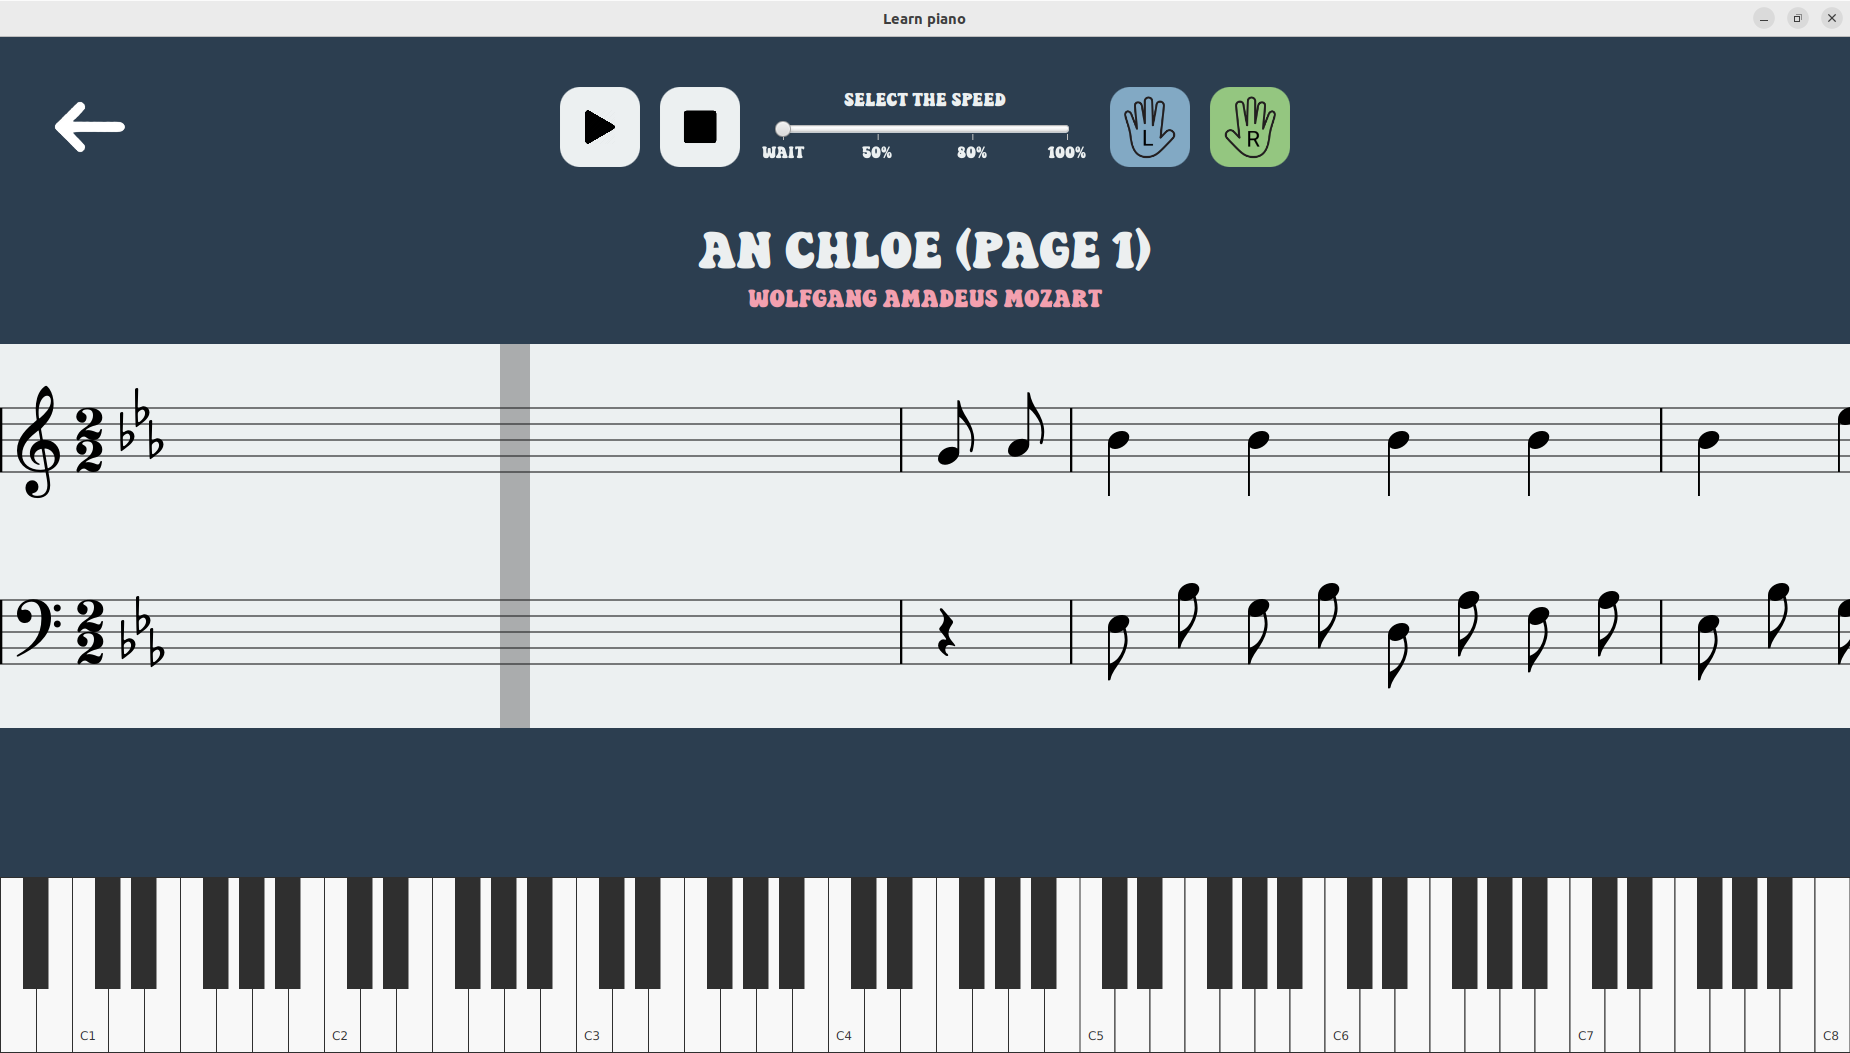
\includegraphics[width=\textwidth]{main-screen.png}
	\caption{Glavni zaslon aplikacije}
	\label{fig:mainscreen}
\end{figure}

Prvi gumb u alatnoj traci služi za pokretanje i pauziranje reprodukcije. Kada pjesma nije u reprodukciji, gumb prikazuje ikonu za početak reprodukcije, što je vidljivo na slici \ref{fig:mainscreen}. Tijekom reprodukcije, gumb prikazuje ikonu za pauziranje, vidljivu na slici \ref{fig:mainplaying}.

\begin{figure}[H]
	\centering
	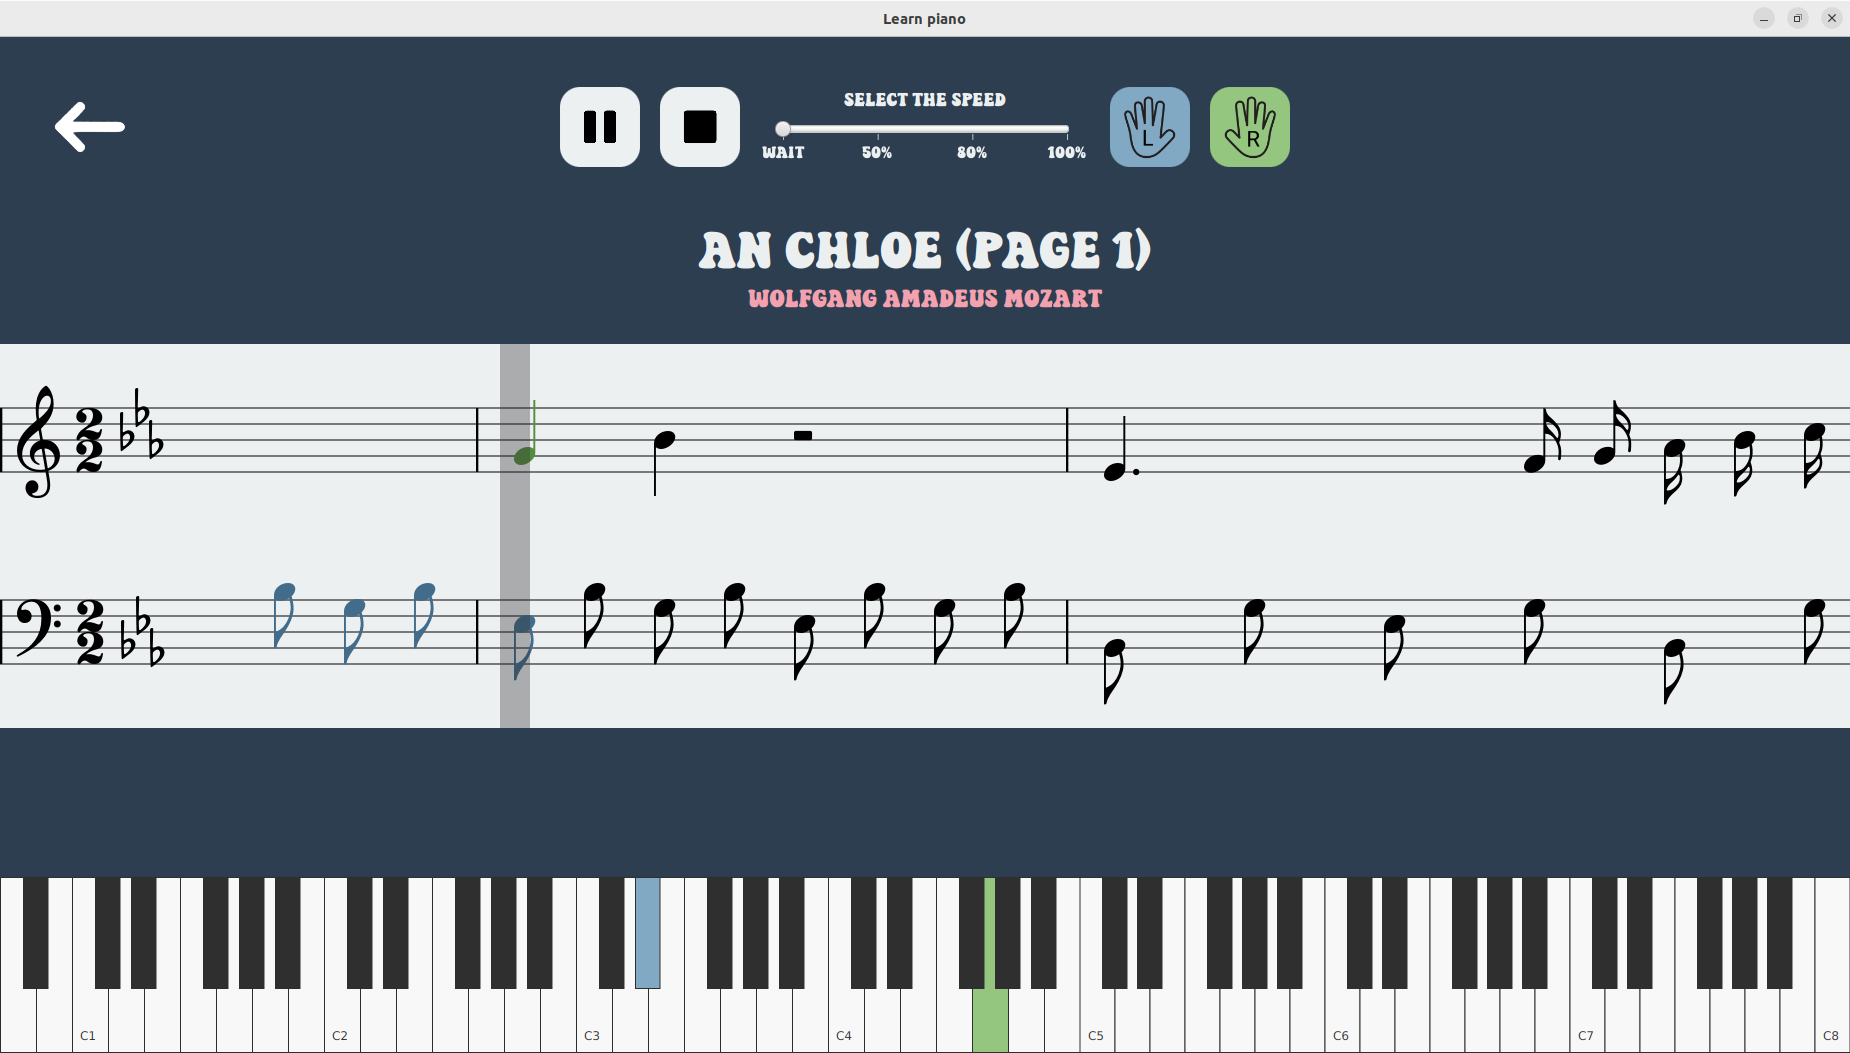
\includegraphics[width=\textwidth]{main-playing.png}
	\caption{Glavni zaslon aplikacije za vrijeme reprodukcije}
	\label{fig:mainplaying}
\end{figure}

Sljedeći gumb služi za zaustavljanje reprodukcije, što uključuje pauziranje i vraćanje notnog zapisa na početak, odnosno resetiranje reprodukcije. 

U sredini alatne trake nalazi se klizač (engl. \textit{slider}) za odabir brzine reprodukcije. Prva opcija, a ujedno i zadana, označena je oznakom \textit{Wait} i omogućuje reprodukciju gdje aplikacija čeka da korisnik odsvira točne tipke, dok se prijelazi između odsviranih nota odvijaju normalnom brzinom. Ostale tri opcije klizača su \textit{50\%}, \textit{80\%} i \textit{100\%}, što označava različite brzine reprodukcije. Kod početka učenja pjesme, sporija reprodukcija može olakšati praćenje, dok će napredniji korisnici moći svirati punom brzinom.

Zadnja dva gumba alatne trake služe za odabir ruke koju se želi vježbati. Sviranje svake ruke zasebno olakšava proces učenja, jer omogućuje fokusiranje na tehniku i točnost svake ruke posebno prije nego što se pređe na zajedničko sviranje. U slučaju da se pjesma svira samo jednom rukom, ti gumbi se neće prikazati, kao što je prikazano na slici \ref{fig:mainonehand}, i tada se drugo crtovlje također ne prikazuje.

\begin{figure}[h]
	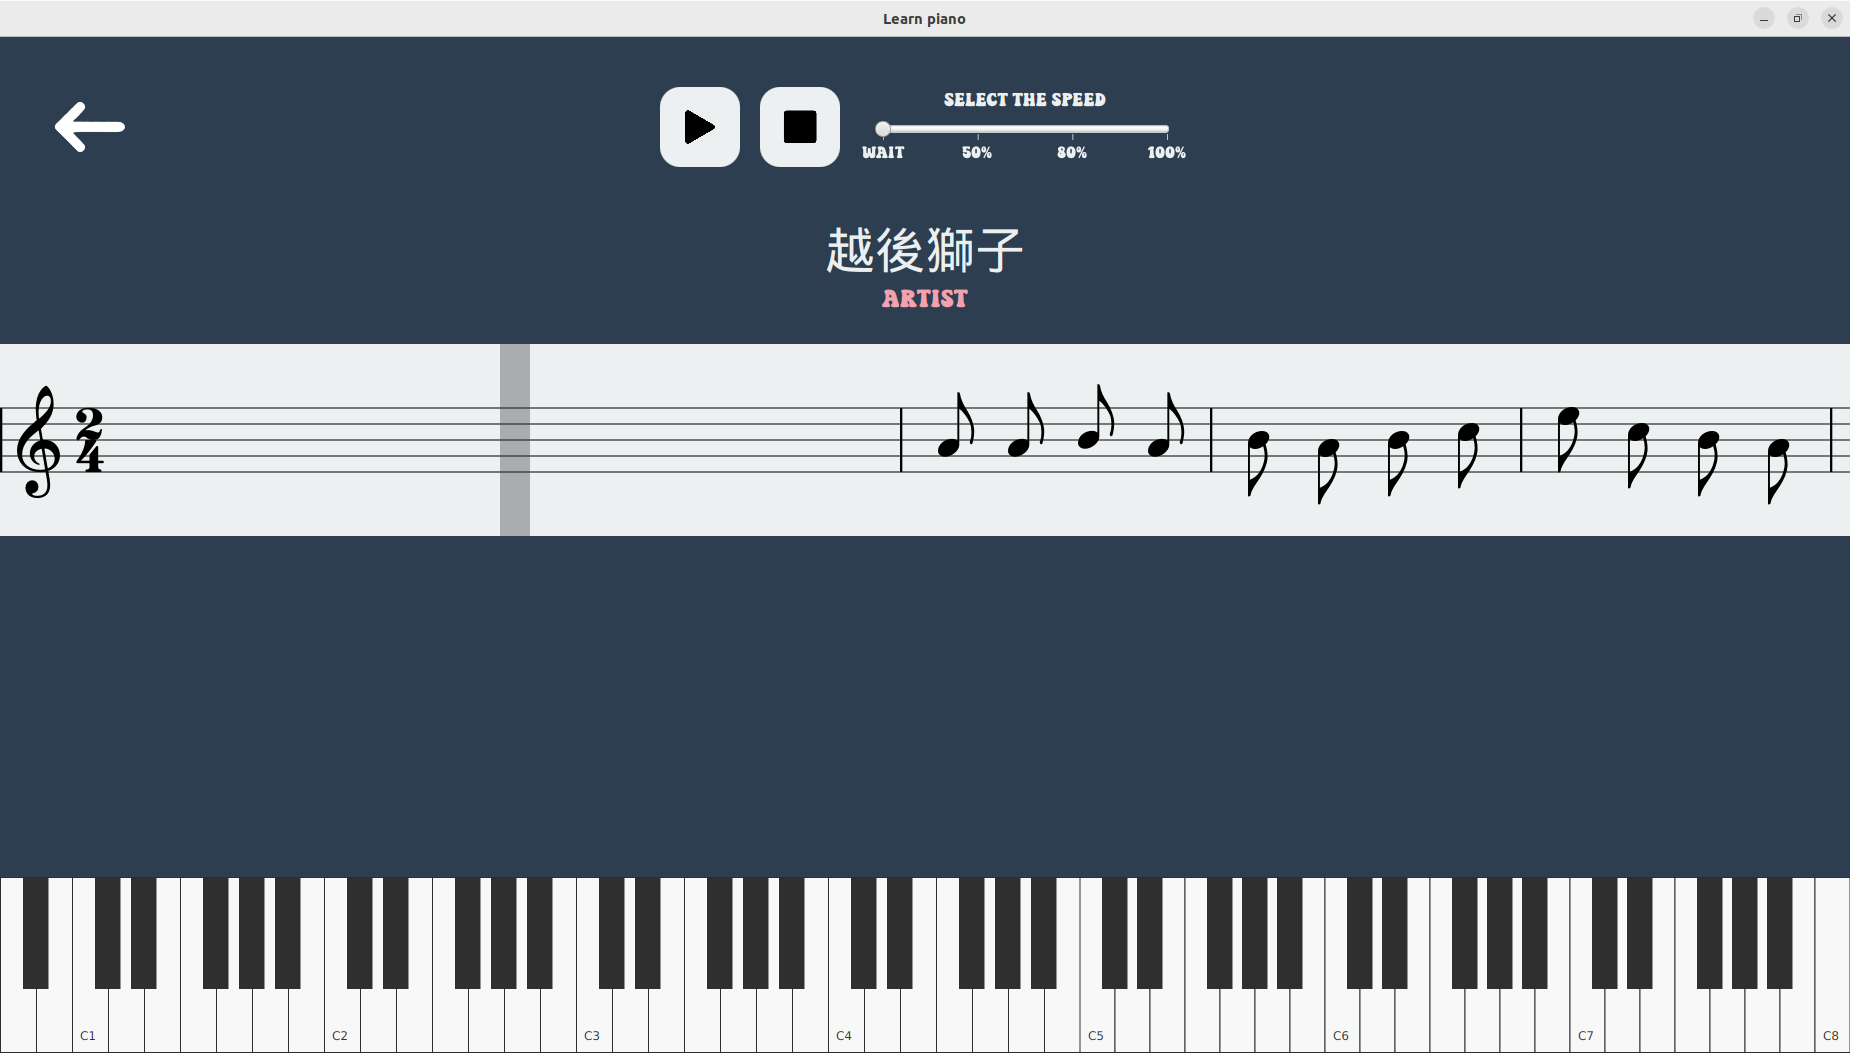
\includegraphics[width=\textwidth]{main-one-hand.png}
	\centering
	\caption{Glavni zaslon kad pjesma sadrži note za samo jednu ruku}
	\label{fig:mainonehand}
\end{figure}

Kada je pjesma koja sadrži note za obje ruke prikazana, oba gumba su aktivna, što se može vidjeti na slici \ref{fig:mainscreen}, gdje je gumb za lijevu ruku obojen plavo, a gumb za desnu ruku zeleno. Isključivanjem jedne od ruku, gumb te ruke postaje bijeli, a crtovlje za tu ruku više se ne prikazuje. Na slici \ref{fig:mainrighthand} prikazano je kako izgleda kad je lijeva ruka isključena, pa se prikazuje samo crtovlje za desnu ruku. Ako bi desna ruka bila isključena, prikazalo bi se samo crtovlje za lijevu ruku, koje bi se automatski pomaknulo na mjesto crtovlja desne ruke, odnosno pozicioniralo više.

\begin{figure}[h]
	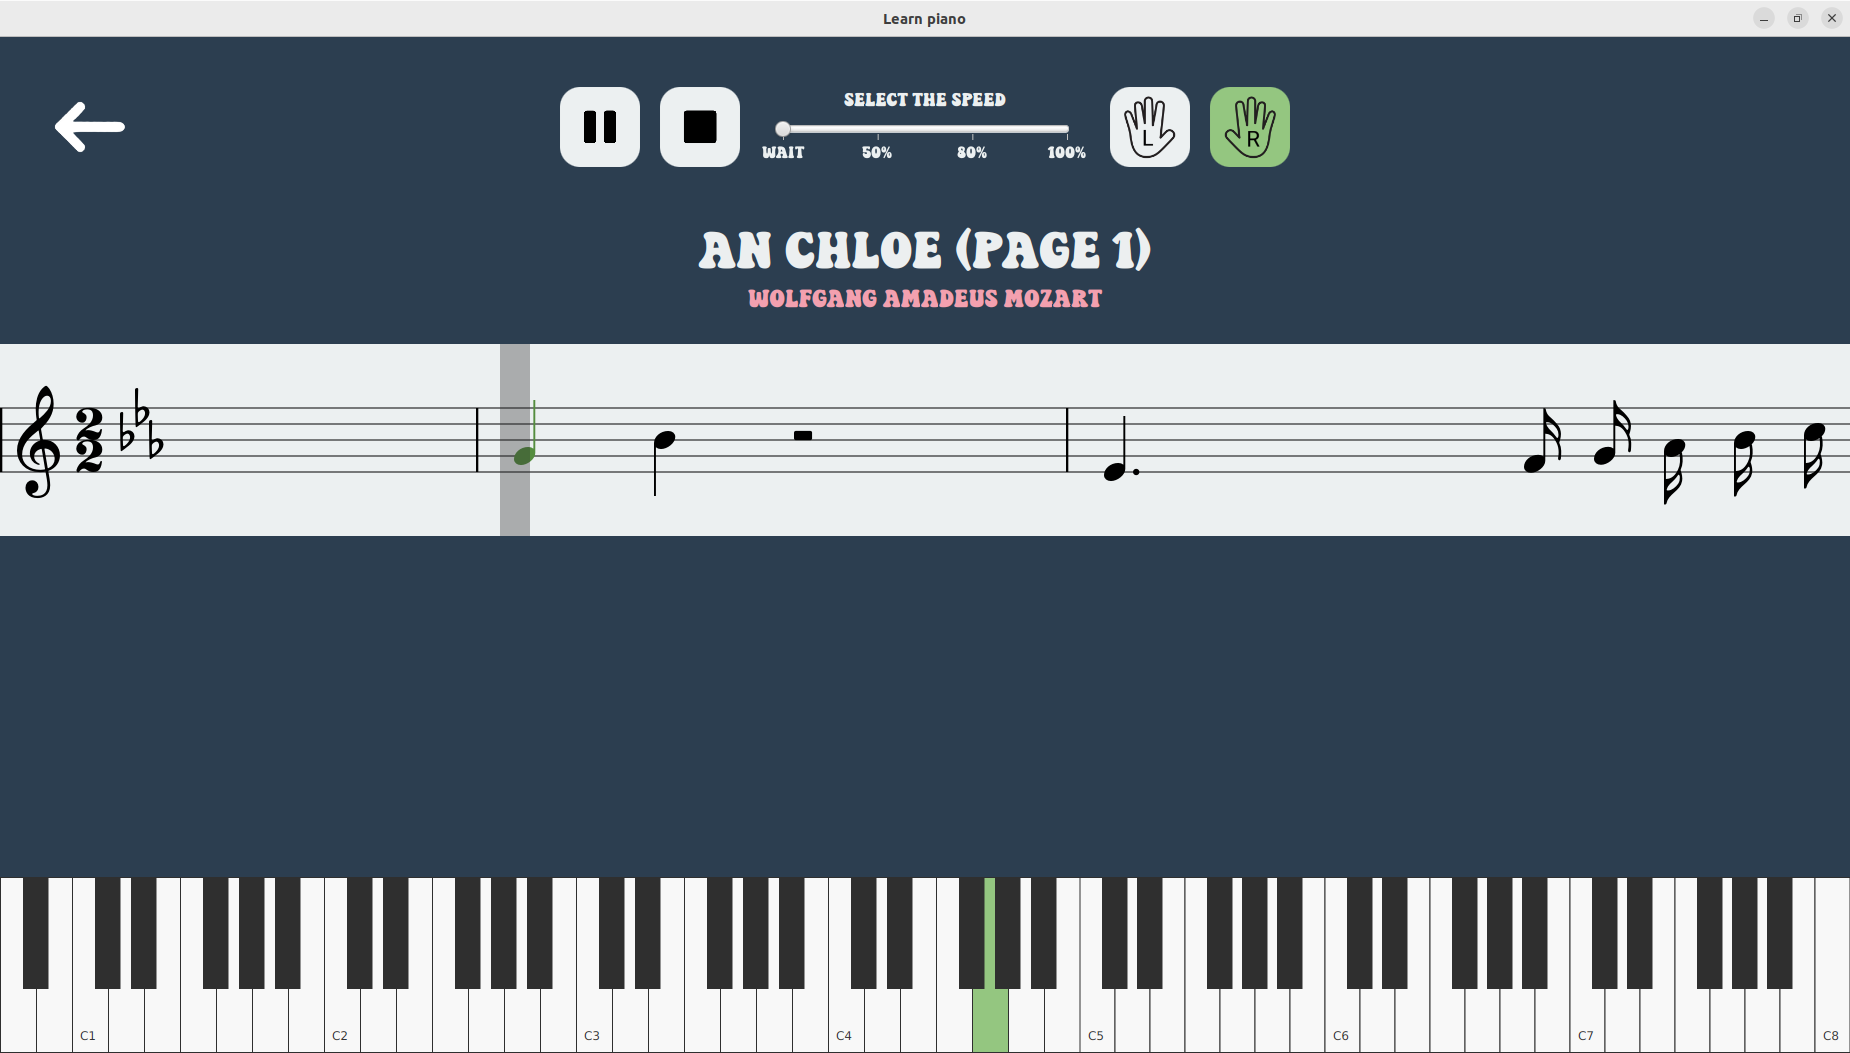
\includegraphics[width=\textwidth]{main-right-hand.png}
	\centering
	\caption{Glavni zaslon kad pjesma sadrži note za samo jednu ruku}
	\label{fig:mainrighthand}
\end{figure}

Alatnom trakom upravlja kontroler \textit{PlayViewController}, koji također nadzire cijeli zaslon. Ovaj kontroler prima korisničke akcije iz alatne trake i prosljeđuje odgovarajuće upute dalje. Uz njega, na upravljanju glavnim zaslonom sudjeluju još dva kontrolera: \textit{SheetMusicController}, koji upravlja notnim zapisom, i \textit{PianoKeyboardController}, koji kontrolira prikaz klavijature.

\subsection{Notni zapis}
U sredini zaslona nalazi se notni zapis. Ispod notnog zapisa, a iznad alatne trake, prikazani su naziv pjesme i ime autora. Ovi podaci u MusicXML datoteci nalaze se u zaglavlju koje sadrži različite metapodatke. Naziv pjesme može se pronaći na dva mjesta: unutar oznake \textit{<movement-title>} ili u oznaci \textit{<work-title>}, koja je smještena unutar oznake \textit{<work>}, a aplikacija ih oba uzima u obzir.

Oznaka \textit{<creator>} u MusicXML dokumentu, smještena unutar oznake \textit{<identification>}, koristi se za označavanje osoba koje su doprinijele stvaranju skladbe. Može se koristiti za označavanje različitih uloga, poput kompozitora, tekstopisca ili aranžera, putem atributa \textit{type} (npr. \textit{composer, lyricist, arranger}). Unutar oznake \textit{<creator>} navodi se ime osobe koja je ispunila tu ulogu. Budući da se uloga \textit{composer} pojavljuje u gotovo svim MusicXML dokumentima, bilo da se radi o klasičnim skladbama ili modernim pjesmama, ime navedeno u ovoj oznaci prikazuje se kao autor pjesme na zaslonu.

Ispod naslova pjesme nalazi se notni zapis, koji može sadržavati jedan ili dva dijela (crtovlja), ovisno o tome izvodi li se skladba s jednom ili dvije ruke. Svaki dio notnog zapisa sastoji se od četiri elementa. Prvi element je notno crtovlje, koje se sastoji od pet horizontalnih linija na kojima se prikazuju note i druge glazbene oznake.

\subsubsection{Određivanje atributa}
Drugi element odnosi se na stalne atribute pjesme koji se nalaze na lijevom kraju crtovlja, čija se pozicija i vrijednosti ne mijenjaju tijekom izvođenja. Ovi atributi uključuju osnovne informacije o pjesmi, kao što su ključ, mjera i tonalitet (prikazan kroz povisilice i snizilice), a nalaze se na početku notnog zapisa.

Svi ovi atributi mogu se pronaći unutar oznake \textit{<attributes>} u MusicXML datoteci. Ova oznaka smještena je unutar prvog takta klavirskog dijela skladbe. Primjer strukture oznake \textit{<attributes>} prikazan je na slici \ref{fig:attributesxml}, dok je njen odgovarajući notni zapis generiran u aplikaciji prikazan na slici \ref{fig:attributessheet}.

\begin{figure}[h]
	\centering
	\begin{minipage}{0.49\textwidth}
		\centering
		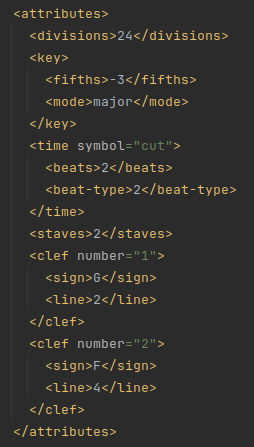
\includegraphics[width=\linewidth]{attributes-xml.png}
		\caption{Atributi u MusicXML datoteci}
		\label{fig:attributesxml}
	\end{minipage}
	\hfill
	\begin{minipage}{0.42\textwidth}
		\centering
		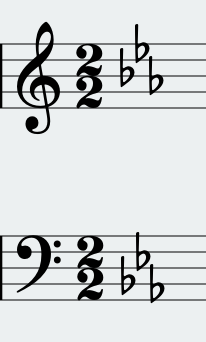
\includegraphics[width=\linewidth]{attributes-sheet.png}
		\caption{Notni zapis atributa u aplikaciji}
		\label{fig:attributessheet}
	\end{minipage}
	\caption{Primjer atributa skladbe}
\end{figure}

Prvi element \textit{<divisions>}, s vrijednošću 24, definira relativno trajanje četvrtinke. Iako ova oznaka nije izravno vezana za atribute na početku notnog zapisa, od ključne je važnosti za kasniji izračun tempa. Slijedi oznaka \textit{<key>}, koja određuje tonalitet skladbe i sadrži dva podelementa. Prvi \textit{<fifths>}, označava broj povisilica (ako je vrijednost pozitivna) ili snizilica (ako je vrijednost negativna) u tonalitetu. Drugi element \textit{<mode>}, određuje je li tonalitet durski (engl. \textit{major}) ili molski (engl. \textit{minor}). U ovom primjeru, vrijednost \textit{fifths} iznosi -3, što znači da tonalitet sadrži tri snizilice. U kombinaciji s vrijednošću \textit{major}, to označava tonalitet E$\flat$-dur.

Tonalitet je sustav organizacije tonova u skladbi, gdje se svi tonovi usmjeravaju prema tonici, glavnom tonu. Ovisno o ljestvici, tonalitet može biti durski (vedar) ili molski (tamniji). Prepoznaje se prema predznacima (povisilicama $\sharp$ i snizilicama $\flat$) iza ključa u notnom zapisu, koji pokazuju povišene ili snižene tonove. Na primjer, C-dur i njegov paralelni a-mol nemaju predznake, dok G-dur ima jednu povisilicu (F$\sharp$). Postoji 30 različitih tonaliteta, ali zbog enharmonije neki zvuče isto, iako imaju različite nazive (npr. C$\sharp$-dur i D$\flat$-dur). Zbog toga se zapravo koristi 24 različita tonaliteta, 12 durskih i 12 molskih, prikazanih na slici \ref{fig:fifths}.

\begin{figure}[h]
	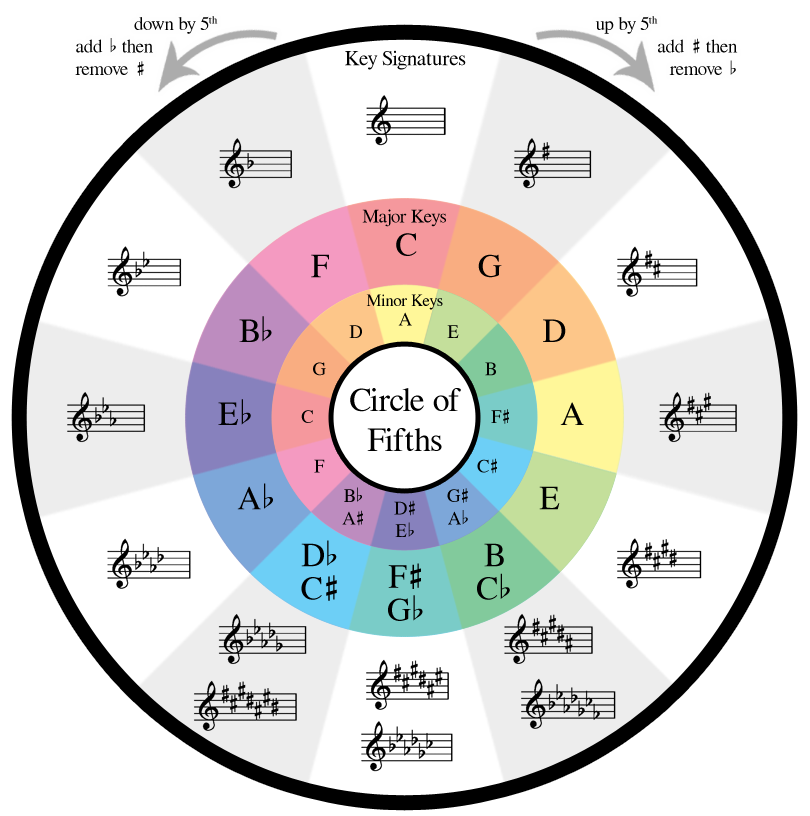
\includegraphics[scale=1.8]{fifths.png}
	\centering
	\caption{Prikaz kvintnog i kvartnog kruga \cite{fifths}}
	\label{fig:fifths}
\end{figure}

Tonaliteti se organiziraju u kvintni (pomak za kvintu dodaje povisilice) i kvartni krug (pomak za kvartu dodaje snizilice). Ova dva kruga su blisko povezana, jer se do istog tonaliteta može doći pomakom kvinte unatrag ili kvarte unaprijed. Na primjer, C-dur prelazi u F-dur pomakom kvarte unaprijed ili kvinte unatrag. Zbog toga se često spominje samo kvintni krug, gdje se pomaci u oba smjera prikazuju jednom vrijednošću s pozitivnim ili negativnim predznakom, kao što je to slučaj u MusicXML formatu.

Oznaka \textit{<time>} definira mjeru pomoću dva elementa. Element \textit{<beats>} određuje broj udaraca (engl. \textit{beat}) i odgovara brojnika mjere, dok element \textit{<beat-type>} određuje vrstu udarca (npr. 2 za polovinku, 4 za četvrtinku) i predstavlja nazivnik mjere. U ovom primjeru riječ je o dvopolovinskoj mjeri (2/2).

Oznaka \textit{<staves>} s vrijednošću 2 označava da skladba koristi dva notna crtovlja, a detaljnije je objašnjena u pododjeljku \ref{sec:formats}.

Oznaka \textit{<clef>} koristi se za određivanje ključa u notnom zapisu, pri čemu je podelement \textit{<sign>} ključan za identifikaciju. Vrijednost ovog elementa određuje tip ključa pri čemu se najčešće koriste: \textit{G} za violinski ključ i \textit{F} za bas ključ, oba koja su korištena u ovom radu. Podelement \textit{<line>} određuje na kojoj liniji notnog crtovlja se ključ postavlja. Violinski ključ (\textit{G}) se standardno nalazi na drugoj liniji od dna, dok je bas ključ (\textit{F}) smješten na četvrtoj liniji, kao što je i u primjeru.

Ako neki od ovih atributa nije naveden postavlja se na zadane postavke: \textit{divisions} na 8, \textit{fifths} na 0, \textit{beats} na 4, \textit{beat-unit} na 4, \textit{staves} na 1 i \textit{sign} na G.

\subsubsection{Određivanje i pozicioniranje notnog zapisa}
Desno od atributa na notnom crtovlju nalazi se ostatak notnog zapisa koji sadrži same note. Korijenski element MusicXML datoteke, \textit{<score-partwise>}, koji koristi moja aplikacija, organizira sadržaj u popis dijelova (\textit{<part>}), od kojih jedan mora biti namijenjen klaviru. Element \textit{<part>} sastoji se od niza elemenata \textit{<measure>}, koji su vremenski poredani. Svaki \textit{<measure>} element predstavlja jedan takt, što je osnovna ritmička jedinica u glazbi. Moja aplikacija na sličan način organizira note po taktovima i prikazuje ih na ekranu. Primjer strukture jednog takta u MusicXML formatu prikazan je na slici \ref{fig:measurexml}, dok se odgovarajući notni zapis može vidjeti na slici \ref{fig:measuresheet}.

\begin{figure}[h]
	\centering
	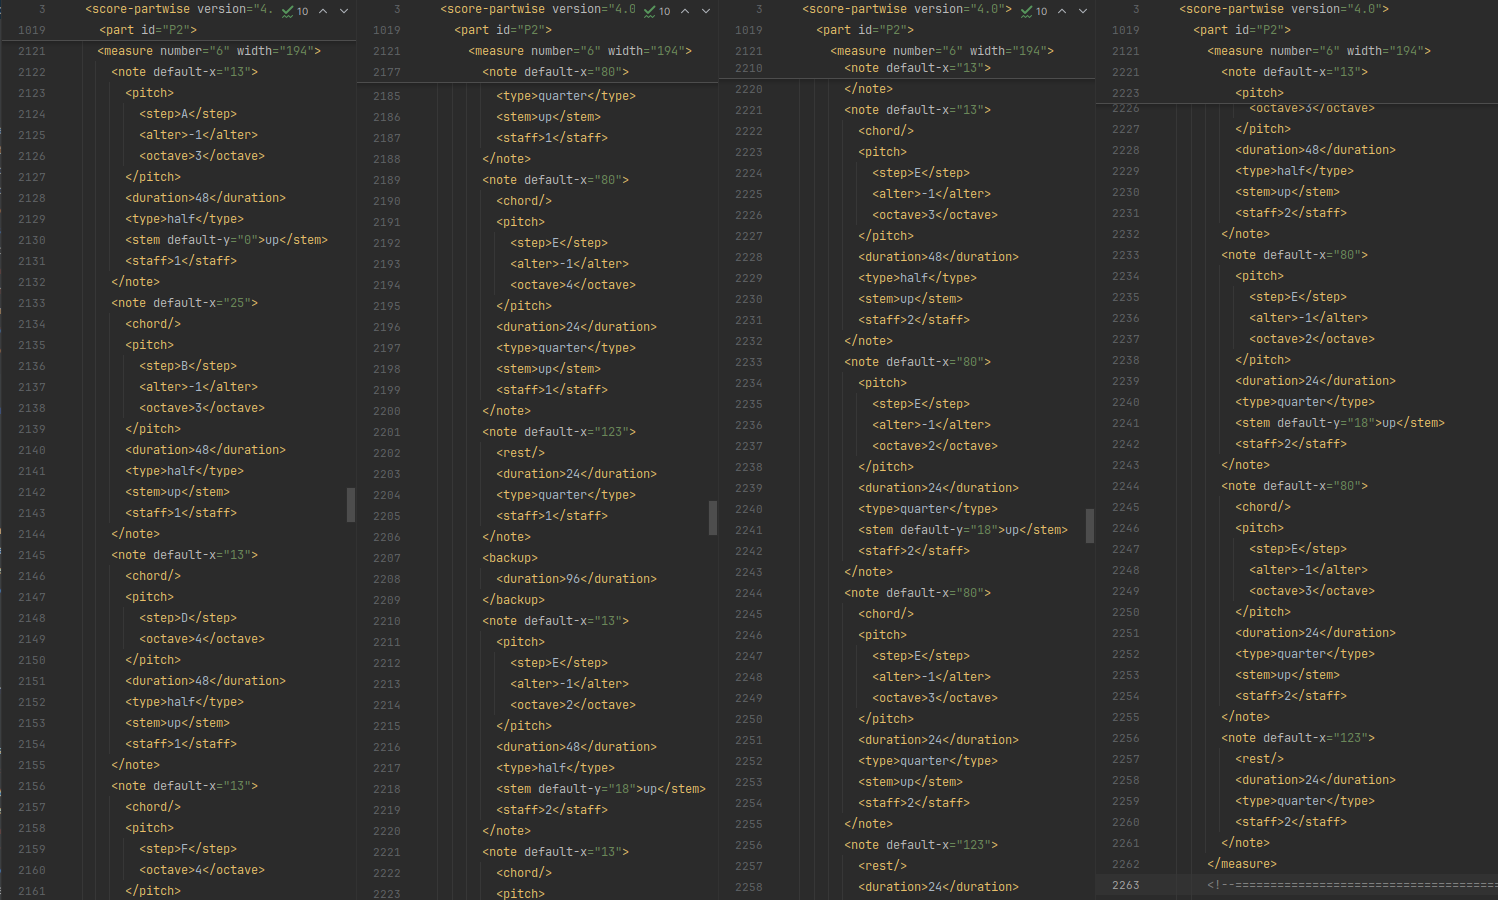
\includegraphics[width=\linewidth]{measure-xml.png}
	\caption{Prikaz takta u MusicXML datoteci}
	\label{fig:measurexml}
	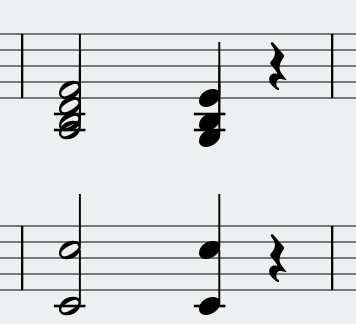
\includegraphics[scale=0.54]{measure-sheet.png}
	\caption{Prikaz takta u aplikaciji}
	\label{fig:measuresheet}
\end{figure}

Element \textit{<measure>} može sadržavati razne podelemente, poput \textit{<attributes>}, ali dva ključna za prezentaciju takta u mom slučaju su \textit{<note>} i \textit{<backup>}. Kako bih pojednostavila prikaz i praćenje reprodukcije taktova, kreirala sam razred \textit{MeasurePairModel}. Ovaj model uključuje listu nota za desnu i, ukoliko se koristi, listu za lijevu ruku. Budući da su taktovi u obje ruke jednake širine i trajanja, taj model također sadrži informacije o tim parametrima.

\textit{MeasurePairModel} ne pohranjuje izravno listu nota, već listu objekata tipa \textit{MusicNodeModel}. Ovaj objekt obuhvaća sve note, kao i dodatne elemente, poput pomoćnih crta, koje se sviraju istovremeno. Na primjeru prikazanom na slici \ref{fig:measuresheet}, u gornjem crtovlju prikazan je prvi akord. Taj akord je predstavljen jednim objektom \textit{MusicNodeModel}, koji sadrži četiri note i dvije pomoćne crte, što ukupno čini šest objekata tipa \textit{NoteModel}.

\begin{figure}[h]
	\centering
	\begin{minipage}{0.55\textwidth}
		\centering
		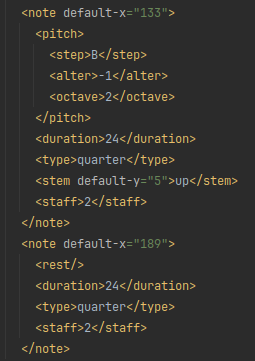
\includegraphics[width=\linewidth]{notes-xml.png}
		\caption{Primjer note i pauze u MusicXML datoteci}
		\label{fig:notesxml}
	\end{minipage}
	\hfill
	\begin{minipage}{0.35\textwidth}
		\centering
		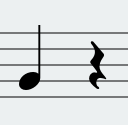
\includegraphics[width=\linewidth]{notes-sheet.png}
		\caption{Notni zapis note i pauze}
		\label{fig:notessheet}
	\end{minipage}
	\caption{Primjer note i pauze}
\end{figure}

\textit{NoteModel} predstavlja bilo koji element notnog zapisa, bilo da se radi o notama, pauzama ili drugim pomoćnim elementima. Na slici \ref{fig:notesxml} prikazan je MusicXML zapis jedne note i jedne pauze, dok je na slici \ref{fig:notessheet} prikazana ista nota i pauza u notnom zapisu unutar aplikacije.

Note uključuju element \textit{<pitch>}, koji određuje visinu tona koristeći tri svojstva: ton unutar oktave (\textit{<step>}), broj oktave (\textit{<octave>}) te opcionalno predznak (\textit{<alter>}), gdje je -1 predznak za sniženi ton, a 1 za povišeni. U prethodnom primjeru radi se o tonu H$\flat$2 (engl. B$\flat$2). Budući da je pjesma napisana u tonalitetu koji već uključuje sniženi ton H, na notnom crtovlju nije dodatno označeno sniženje.

Note mogu opcionalno imati oznaku \textit{<stem>} s vrijednostima \textit{up} ili \textit{down}, koja određuje smjer drške note – prema gore ili dolje. Pauze se označavaju korištenjem elementa \textit{<rest/>}.

Sljedeća tri elementa zajednička su za note i za pauze. Element \textit{<duration>} označava relativno trajanje note ili pauze, \textit{<type>} definira tip note (npr. q\textit{uarter} za četvrtinku ili četvrtinsku pauzu), a \textit{<staff>} označava crtovlje na kojem se nota ili pauza nalazi. U prikazanom primjeru, broj 2 označava drugo crtovlje, odnosno ono za lijevu ruku.

Note unutar takta pozicioniraju se uzimajući u obzir najkraću notu u taktu. Note te duljine smještaju se na jediničnu udaljenost jedna od druge, dok su ostale note raspoređene proporcionalno njihovom trajanju. Ovaj pristup osigurava ravnomjeran vizualni ritam notnog zapisa, omogućujući da se zapis pomiče ujednačenom brzinom tijekom reprodukcije takta. Reprodukcija pjesme, odnosno pomicanje notnog zapisa ulijevo, odvija se brzinom koja ovisi o tempu skladbe i širini takta. Budući da postoji dodatna udaljenost između početka takta i prve note, prijelaz između zadnje note prethodnog takta i prve note sljedećeg takta vizualno se čini bržim.

\subsubsection{Kontrolna linija}
Četvrti element notnog crtovlja je kontrolna linija, prozirno sive boje, koja se proteže preko oba crtovlja i služi kao orijentir za sviranje nota. Svaki takt sadrži slušač (engl. \textit{listener}), čija je uloga obavještavanje \textit{PianoKeyboardControllera} o tome kada treba odsvirati ili prekinuti sviranje određenih nota.

Kada objekt \textit{MusicNodeModel} uđe u područje kontrolne linije, a note još nisu odsvirane, slušač tog takta detektira ovaj događaj i obavještava sustav o notama koje treba odsvirati. U tom trenutku te se note označuju kao odsvirane, kako bi se izbjeglo njihovo ponovno aktiviranje. Neposredno prije nego što \textit{MusicNodeModel} uđe u kontrolnu liniju, aktivira se drugi slušač, zadužen za obavještavanje o prekidu sviranja prethodnih nota, kako bi se sustav mogao pripremiti za nadolazeće note.

\subsection{Klavijatura}
\label{sec:keyboard}
Na dnu zaslona nalazi se prikaz klavijature, koja obuhvaća cijeli raspon koncertnog klavira, od A0 do C8. Veličina klavijature dinamički se prilagođava širini prozora, osiguravajući optimalan prikaz bez obzira na veličinu zaslona. Klavirske tipke implementirane su kao instance razreda \textit{Rectangle} iz JavaFX biblioteke. Radi lakšeg snalaženja, tipke s tonom C sadrže oznaku na dnu, a uz to je na njima ispisan i broj oktave.

Tijekom reprodukcije skladbe, tipke koje treba odsvirati ističu se drugačijom bojom. Na slici \ref{fig:keyboardnotplayed} prikazan je izgled istaknutih tipki prije nego što ih korisnik odsvira. Tipke koje se sviraju lijevom rukom označene su plavom bojom, dok su tipke za desnu ruku označene zelenom. Kako bih osigurala lakše praćenje, te su boje dosljedno korištene u cijeloj aplikaciji, uključujući gumbe za odabir ruke i prikaz odsviranih nota na notnom zapisu.

\begin{figure}[h]
	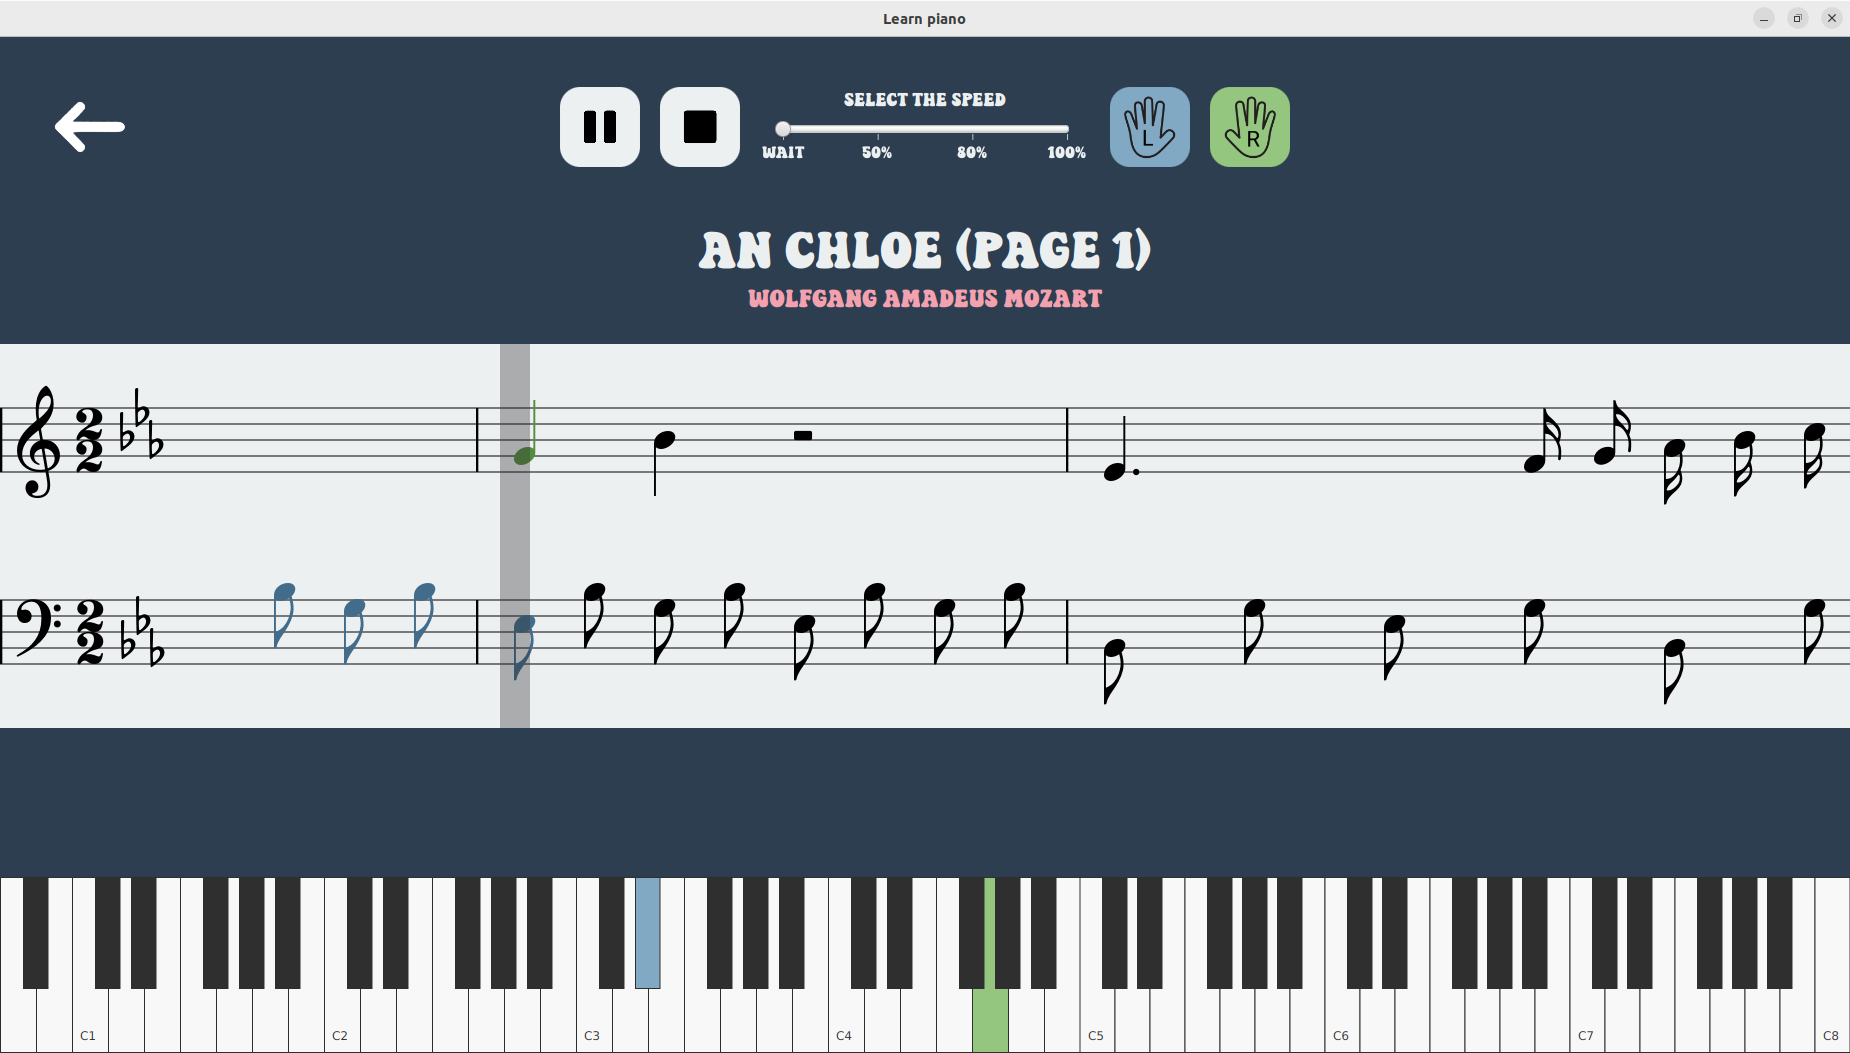
\includegraphics[width=\linewidth]{main-playing.png}
	\centering
	\caption{Prikaz istaknutih tipki na klavijaturi dok se ne sviraju}
	\label{fig:keyboardnotplayed}
\end{figure}

Kada korisnik pritisne ispravne tipke, one promijene boju na tamniju, što se može vidjeti na slici \ref{fig:keyboardplayed}. Pritisnuta je tipka G4, te je promijenila boju u tamno zelenu. Ako korisnik otpusti ispravnu tipku, a nota još nije završila sa sviranjem, boja tipke vraća se na svjetliju varijantu.

\begin{figure}[h]
	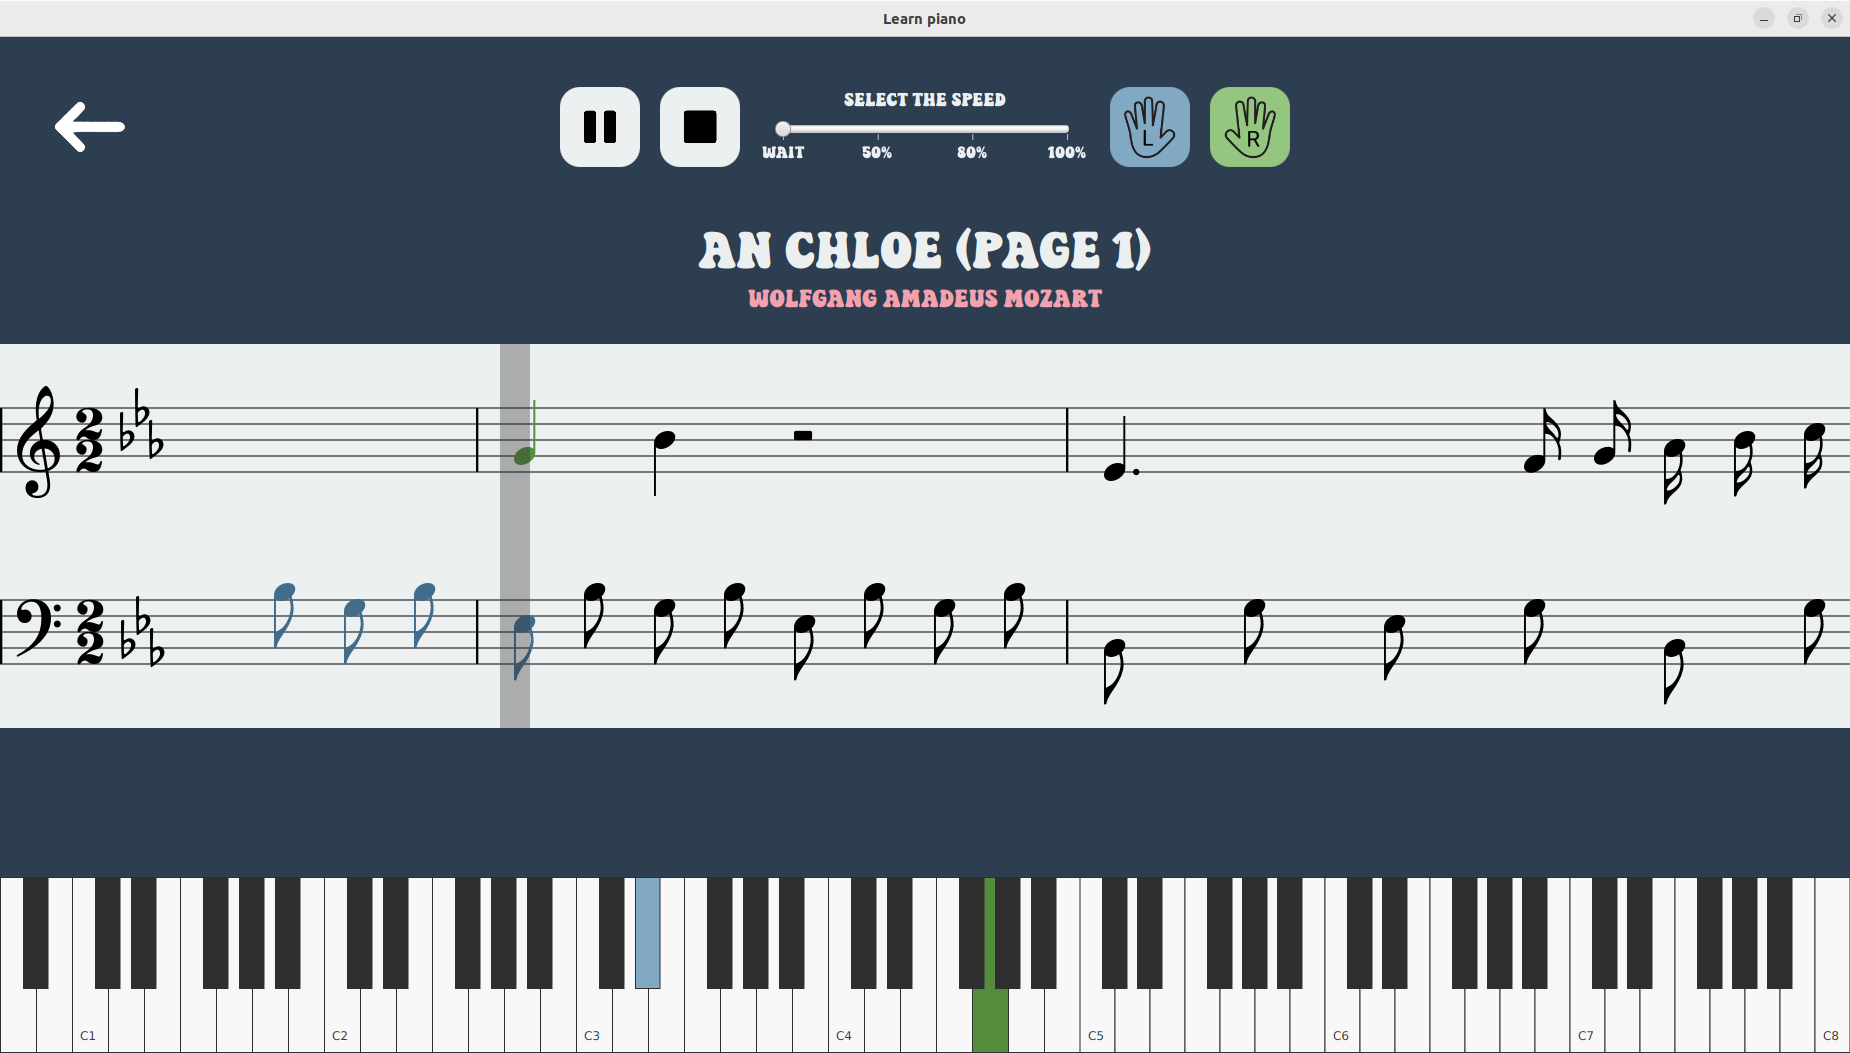
\includegraphics[width=\linewidth]{keyboard-played.png}
	\centering
	\caption{Prikaz istaknutih tipki na klavijaturi za vrijeme sviranja}
	\label{fig:keyboardplayed}
\end{figure}

Pritisak tipki koje se ne sviraju u tom trenutku ne prikazuje se na klavijaturi. Kada nota završi, boja pripadajuće tipke odmah se vraća u normalno stanje. Upravljanje bojama tipki obavlja \textit{PianoKeyboardController}, koji također upravlja zvučnom reprodukcijom skladbe putem singleton razreda \textit{MidiPlayback}.

Razred \textit{MidiPlayback} odgovoran je za otvaranje MIDI kanala i slanje MIDI poruka za reprodukciju. Proces otvaranja kanala uključuje sljedeće korake: prvo se inicijalizira \textit{Synthesizer}, zatim se učitava instrument 0 (klavir), i na kraju se dohvaća prvi kanal. Kod za taj proces prikazan je u nastavku.

\begin{lstlisting}
try {
	synthesizer = MidiSystem.getSynthesizer();
	synthesizer.open();
	Instrument[] instruments = synthesizer.getDefaultSoundbank().getInstruments();
	synthesizer.loadInstrument(instruments[0]);
	channel = synthesizer.getChannels()[0];
	channel.programChange(0);
} catch (MidiUnavailableException ignored) {}
\end{lstlisting}

Kada je kanal otvoren, reprodukcija note ostvaruje se pomoću metode \lstinline|channel.noteOn(midiKey, volume)|, gdje je midiKey numerička vrijednost tipke u rasponu od 0 do 127, a volume predstavlja glasnoću izvedbe u rasponu od 0 do 100. Za zaustavljanje reprodukcije note koristi se metoda \lstinline|channel.noteOff(midiKey)|.

\subsection{Povratna informacija o uspjehu sviranja}
Nakon što korisnik završi sviranje skladbe, otvara se prozor s povratnom informacijom o kvaliteti izvedbe. Prikaz tog prozora može se vidjeti na slici \ref{fig:feedback}, a radi bolje preglednosti, slika je uvećana.

\begin{figure}[h]
	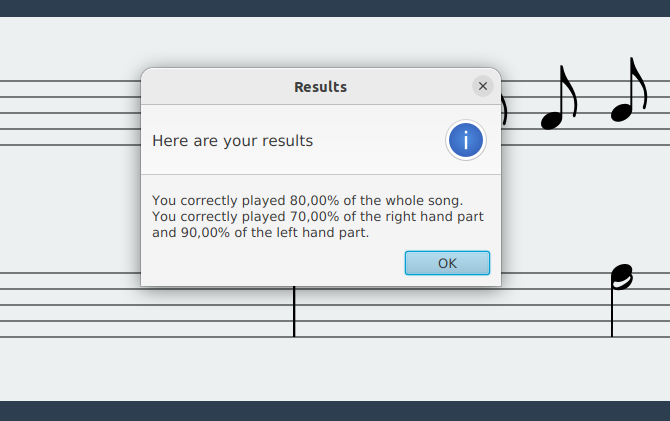
\includegraphics[width=\linewidth]{feedback.png}
	\centering
	\caption{Prikaz prozora s povratnom informacijom}
	\label{fig:feedback}
\end{figure}

Trenutno moja aplikacija prikazuje samo postotak ispravno odsviranih nota. Ako skladba sadrži note za jednu ruku, prikazuje se samo poruka o ukupnoj uspješnosti izvedbe. Međutim, ako skladba uključuje note za obje ruke, prozor prikazuje i detaljne informacije o uspješnosti svake ruke zasebno, uz ukupan rezultat. Tijekom sviranja skladbe, aplikacija prati koje je note korisnik ispravno odsvirao i na temelju toga izračunava postotak uspješnosti.


%---------------------------- Results section -----------------------------

\chapter{Analiza rezultata}
Pokretanjem aplikacije koristeći različite datoteke, uočila sam da notni zapis, a time i prikaz na klavijaturi, nije uvijek jednak očekivanom. Međutim to nije toliki problem, jer da bih pokrila sve mogućnosti notnog zapisa u svojoj aplikaciji, bilo bi potrebno puno više vremena, poznavanja teorije glazbe i iskustva u programiranju.

U odjeljku \ref{sec:results} navesti ću rezultate pokretanja aplikacije, te dobre i loše strane implementacije programa. U odjeljku \ref{sec:improvements} iznijeti ću neke prijedloge za unaprijeđenje i nadogradnju aplikacije u budućnosti. Za prikaz rezultata koristiti ću početak skladbe "An Chloe" skladatelja Wolfganga Amadeusa Mozarta.

\section{Prikaz rezultata}
\label{sec:results}
Ako korisnik učita datoteku koja je u ispravnom formatu, opisanom u pododjeljku \ref{sec:formats}, aplikacija će ispravno funkcionirati. Prema standardu, notni zapis za različite ruke ili crtovlja namijenjen istom instrumentu treba biti unutar istog dijela, dok se razlika između crtovlja označava oznakom \textit{<staff>} unutar svake note. Međutim, mogu se pronaći datoteke koje ne prate ovaj standard, gdje su note za različita crtovlja smještene u različite dijelove. To predstavlja izazov prilikom deserijalizacije dokumenta, a trenutna verzija moje aplikacije ne podržava takav format. Ako korisnik učita takvu datoteku, ona se ili neće učitati – ako nijedan od dijelova ne sadrži naziv "Piano" – ili će prikazivati samo jedno crtovlje, odnosno jednu ruku.

Notni zapis se u većini slučajeva prikazuje ispravno, što je prikazano na slici \ref{fig:eightsapp}. Na toj slici vidi se prikaz jednog takta unutar moje aplikacije. Za usporedbu, na slici \ref{fig:eightssheet} prikazan je isti taj takt u tradicionalnom notnom zapisu. Može se primijetiti da su u aplikaciji sve note ispravno pozicionirane i odgovarajućeg trajanja. Također, pomoćne crte, koje se koriste za prikaz nota izvan standardnog raspona notnog crtovlja, ispravno su prikazane.

\begin{figure}[h]
	\centering
	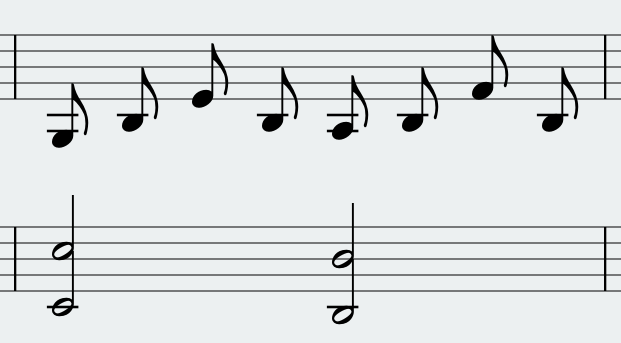
\includegraphics[scale=0.6]{eights-app.png}
	\caption{Prikaz takta u aplikaciji}
	\label{fig:eightsapp}
	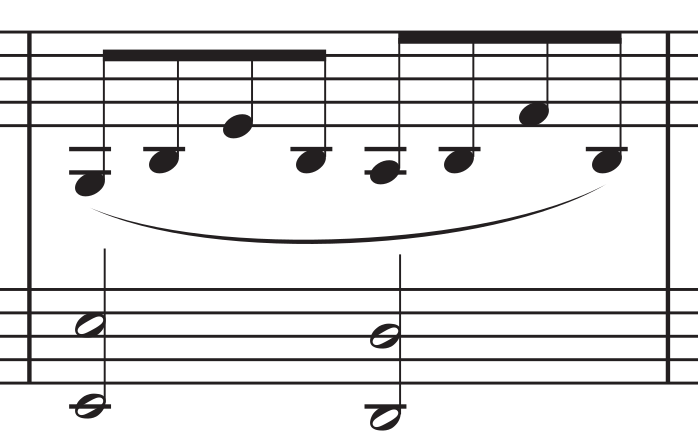
\includegraphics[scale=0.5]{eights-sheet.png}
	\caption{Prikaz takta u postojećem notnom zapisu}
	\label{fig:eightssheet}
\end{figure}

Kada se više osminki ili kraćih nota pojavljuje uzastopno, one se obično povezuju linijama, kao što je prikazano na slici \ref{fig:eightssheet}. U mojoj aplikaciji, međutim, to nisam uspjela implementirati, pa se svaka nota prikazuje odvojeno. Zbog tehničkih ograničenja, nisam mogla koristiti font Bravura za ovu funkcionalnost, pa bi povezivanje nota trebalo ručno nacrtati. U budućnosti smatram da bi bilo korisno implementirati ovu značajku kako bi prikaz bio jasniji korisnicima.

Još jedan problem koji bih željela ispraviti je prikaz osminki i kraćih nota kada su dio akorda. Na slici \ref{fig:eightserror} prikazana su četiri akorda s osminkama, no svaka nota ima svoju vlastitu dršku i zastavicu, što otežava čitljivost zapisa. Umjesto toga, sve note unutar jednog takta trebale bi dijeliti istu dršku s jednom zajedničkom zastavicom, kako bi notni zapis bio jasniji i pregledniji.

\begin{figure}[h]
	\centering
	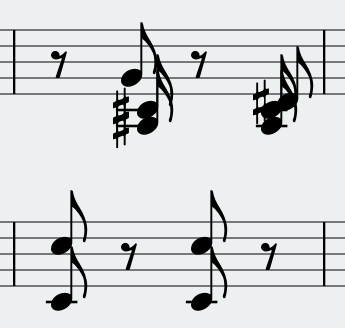
\includegraphics[scale=0.6]{eights-error.png}
	\caption{Prikaz neispravno prikazanih osminki}
	\label{fig:eightserror}
\end{figure}

Također, predznaci ispred nota (npr. povisilice na slici \ref{fig:eightserror}) ne bi smjeli utjecati na položaj same note. Nota bi trebala zadržati svoju uobičajenu poziciju, dok bi se predznak trebao pravilno uskladiti s njom, bez promjene razmaka.

Unatoč ovim problemima, notni zapis se u većini slučajeva ispravno prikazuje, a zvučna reprodukcija i označene tipke na klaviru većinom funkcioniraju kako treba. S obzirom na to da glazba obuhvaća veliki broj različitih elemenata, teško je uvijek uzeti u obzir sve aspekte i osigurati njihovu ispravnu izvedbu.

\section{Mogućnost nadogradnje}
\label{sec:improvements}
S obzirom na ograničeno vrijeme za izradu ovog diplomskog rada, nisam bila u mogućnosti implementirati sve funkcionalnosti koje bih htjela. Iako sam zadovoljna trenutnim stanjem aplikacije i vjerujem da sam uspjela razviti solidan program, svjesna sam da postoji prostor za daljnje nadogradnje. U nastavku ću navesti neke od glavnih funkcionalnosti koje bih voljela uključiti u budućim verzijama aplikacije.

Prva stvar koju bih htjela unaprijediti u aplikaciji je proširenje biblioteke pjesama. Većina sličnih aplikacija nudi velik izbor pjesama različitih razina zahtjevnosti, koje korisnici mogu svirati. Iako bih htjela povećati broj dostupnih pjesama, želim zadržati primarni fokus aplikacije na mogućnosti učitavanja vlastitih datoteka, jer mislim da je to velika prednost ove aplikacije nad mnogima koje već postoje. Međutim, zbog kompleksnosti implementacije te funkcionalnosti, proširenje biblioteke mi nije prioritet.

Prilikom učenja nove skladbe, glazbenici često ne vježbaju od samog početka, već se fokusiraju na određene dijelove kompozicije. Trenutno, moja aplikacija omogućava reprodukciju isključivo od početka skladbe. Zbog toga bih u budućim verzijama željela implementirati mogućnost "navigacije" kroz skladbu, koja bi omogućila reprodukciju od odabranog dijela. Koncept ove funkcionalnosti prikazan je na slici \ref{fig:playhead}, gdje bi korisnici povlačenjem pokazivača mogli odrediti točku od koje žele nastaviti reprodukciju.

\begin{figure}[h]
	\centering
	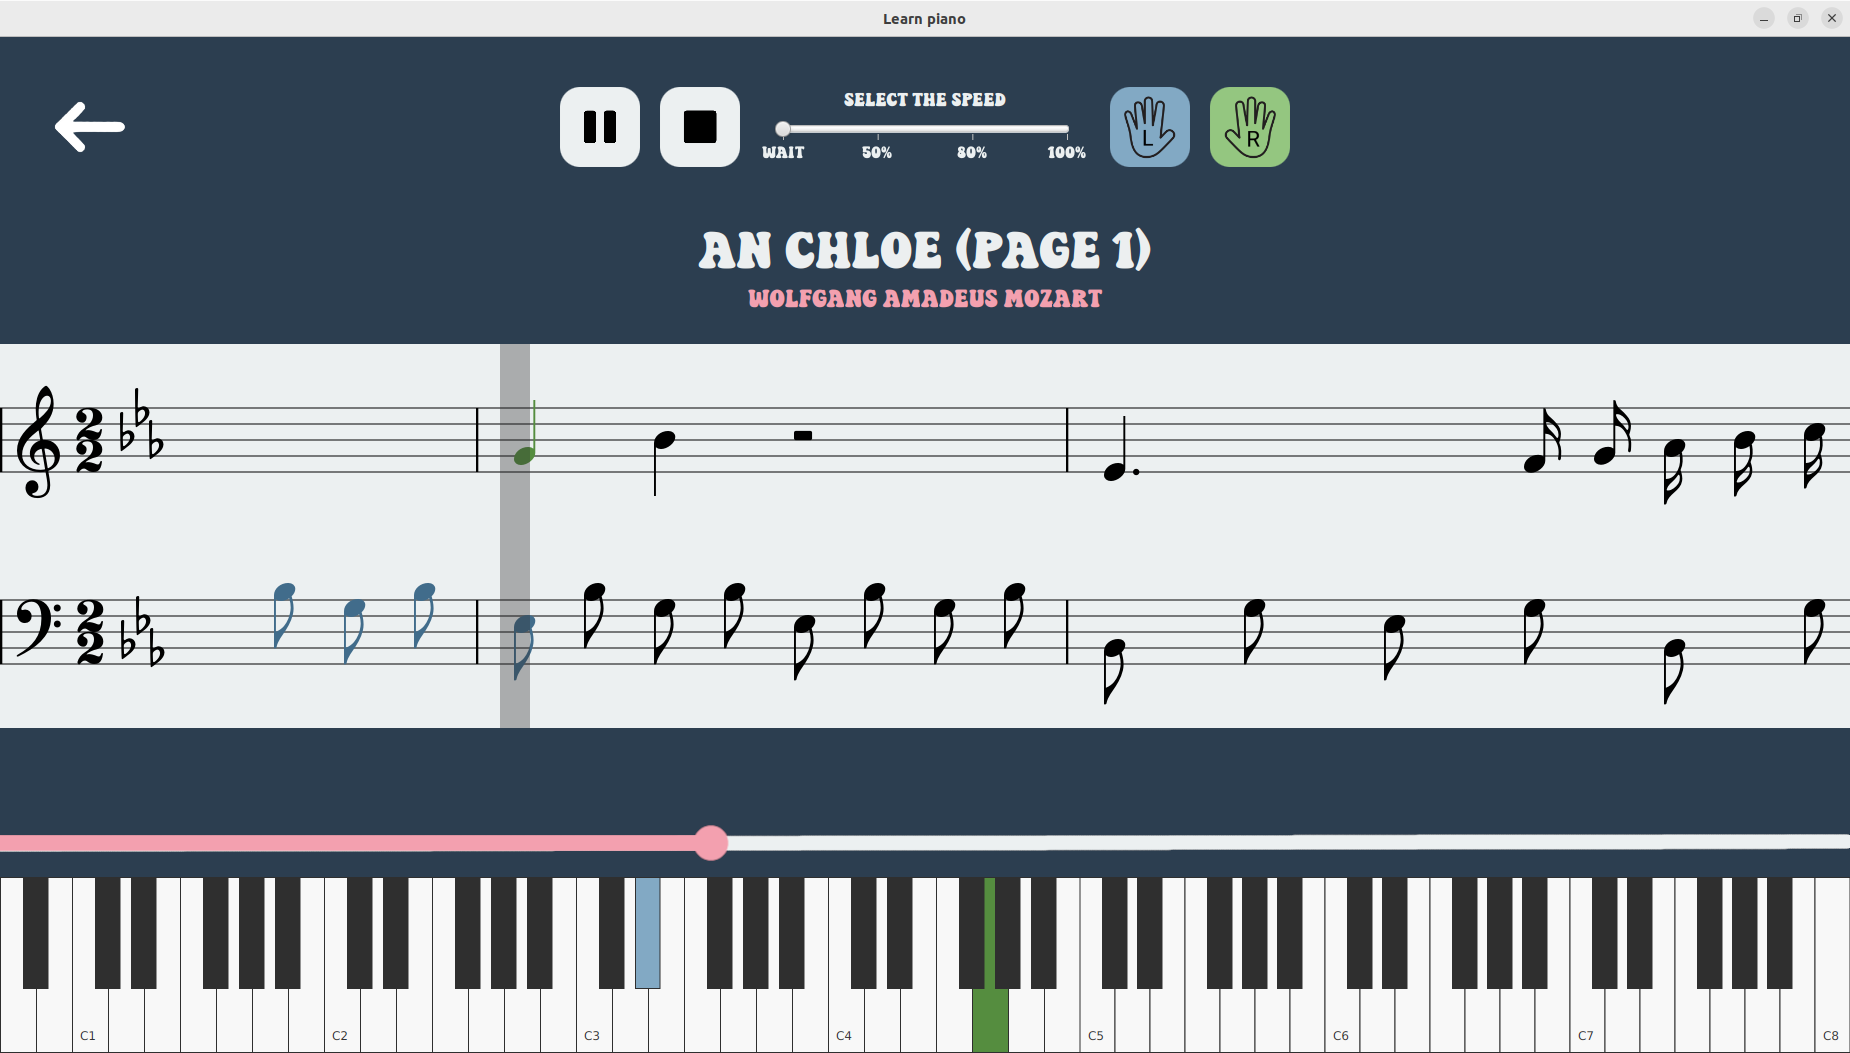
\includegraphics[width=\linewidth]{playhead.png}
	\caption{Ideja prikaza pokazivača reprodukcije}
	\label{fig:playhead}
\end{figure}

Iduća funkcionalnost koju bih željela implementirati je metronom. Metronom pomaže glazbenicima održavati ritam proizvodnjom ritmičkih zvučnih signala. Tijekom pokušaja implementacije, naišla sam na izazov jer nisam uspjela osigurati da metronom radi ispravno. Zbog potrebe za višedretvenošću (engl. \textit{multithreading}), otkucaji metronoma nisu bili sinkronizirani s reprodukcijom i prikazom glazbe. Shvatila sam da, kako bi otkucaji metronoma bili potpuno usklađeni s ostatkom reprodukcije, metronom bi trebao raditi unutar iste dretve i u zajedničkoj petlji s ostatkom koda. Međutim, zbog trenutne strukture aplikacije, ova implementacija nije bila moguća.

S obzirom na to da je u aplikaciji već implementirana zvučna reprodukcija glazbe, dodavanje metronoma moglo bi stvoriti poteškoće glazbenicima pri koncentraciji zbog istovremenog slušanja oba izvora zvuka. Zbog toga mislim da bi optimalno rješenje bilo uvesti dva gumba: jedan za isključivanje metronoma i drugi za isključivanje reprodukcije glazbe. Na taj način, glazbenici bi imali fleksibilnost da sami biraju žele li slušati samo metronom, samo glazbenu reprodukciju, oboje ili nijedno.

Posljednja funkcionalnost koju bih htjela implementirati odnosi se na poboljšanje povratnih informacija o kvaliteti sviranja. Trenutno aplikacija prikazuje samo postotak ispravno odsviranih nota na kraju skladbe, no smatram da bi korisnicima bilo korisno pratiti svoj napredak tijekom vremena. Kako bi se to omogućilo, aplikacija bi trebala pohranjivati podatke o izvedbama, što bi zahtijevalo implementaciju trajne memorije, poput lokalne baze podataka ili integracije s oblakom. Mislim da bi ova funkcionalnost motivirala korisnike na daljnje vježbanje.


%---------------------------- Conclusion section --------------------------

\chapter{Zaključak}
Izrada ove aplikacije omogućila mi je razumijevanje izazova povezanih s primjenom računalnih tehnologija u kreativnim i subjektivnim područjima poput glazbe. Dok računala zahtijevaju preciznost i determinizam, glazba često odstupa od tih pravila, što čini razvoj ovakvih aplikacija relativno zahtjevnim.

Unatoč tim izazovima, uspjela sam razviti aplikaciju koja, iako ne može zamijeniti tradicionalne metode učenja i čitanje pravog notnog zapisa, predstavlja korisno sredstvo za brže i lakše savladavanje novih skladbi. Aplikacija omogućuje korisnicima učenje sviranja klavira na interaktivan i zabavan način, pružajući im mogućnost praćenja napretka i ispravljanja pogrešaka. Iako aplikacija ne može uvijek generirati 100\% točne upute za sviranje, smatram da je izuzetno korisna za one koji žele brzo naučiti željene pjesme, štedeći im vrijeme i trud koji bi inače uložili u učenje čitanja notnog zapisa.

Na kraju, ponosna sam na postignute rezultate i smatram da je ovaj rad značajan doprinos u primjeni računalne tehnologije u glazbenom obrazovanju. Budući da uživam u sviranju klavira i učenju novih pjesama, planiram nastaviti koristiti ovu aplikaciju, što će me potaknuti da ju i dalje unapređujem. Postoje brojne mogućnosti za poboljšanje i nadogradnju koje bih voljela implementirati u budućnosti. Vjerujem da bi ove nadogradnje dodatno povećale funkcionalnost, korisnost i zadovoljstvo korištenja aplikacije. Iako uvijek postoji prostor za napredak, aplikacija koju sam napravila predstavlja dobar temelj za njen daljnji razvoj.

Izvorni kod aplikacije implementirane u sklopu ovoga rada, kao i buduće verzije mogu se pronaći na poveznici \cite{gitrepo}.

%---------------------------- References ----------------------------------

\bibliography{literatura}


%---------------------------- Abstract ------------------------------------

\begin{sazetak}
U ovom radu istraživala sam problem razvoja aplikacije za učenje sviranja klavira, specifično usmjerene na vježbanje izvođenja odabrane skladbe. Razvila sam aplikaciju koja omogućuje korisniku učitavanje željene skladbe u MusicXML formatu, nakon čega aplikacija pomoću pomičnog notnog zapisa i vizualno istaknutih tipki na klaviru prikazuje koje note treba odsvirati. Analizom izvedbe u stvarnom vremenu, aplikacija prati izvedbu korisnika koristeći klavijaturu povezanu s računalom putem MIDI protokola i nudi povratne informacije o točnosti sviranja. Ovaj rad detaljno opisuje razvijenu aplikaciju, uključujući odabrane tehnologije i metode implementacije, te pruža analizu dobivenih rezultata. U radu su također razmotrene mogućnosti za daljnje poboljšanje i nadogradnju aplikacije, s ciljem povećanja njezine funkcionalnosti i prilagodljivosti različitim razinama vještine korisnika.
\end{sazetak}

\begin{kljucnerijeci}
glazba; klavir; midi; musicxml; javafx; desktop aplikacija
\end{kljucnerijeci}

\begin{abstract}
In this thesis, I explored the development of an application designed for learning piano playing, specifically aimed at practicing the performance of selected pieces. I developed an application that allows users to load their chosen piece in MusicXML format, after which the application displays the notes to be played using a scrolling sheet music view and visually highlighted piano keys. By analyzing the performance in real-time, the application evaluates the user's playing using a keyboard connected to the computer via MIDI protocol and provides feedback on the accuracy of the performance. This thesis provides a detailed description of the developed application, including the chosen technologies and implementation methods, and offers an analysis of the obtained results. The thesis also considers possibilities for further improvement and enhancement of the application, with the goal of increasing its functionality and adaptability to different skill levels of users.
\end{abstract}

\begin{keywords}
music; piano; midi; musicxml; javafx; desktop application
\end{keywords}


\end{document}
